\documentclass[12pt]{report}

\usepackage[margin=1in]{geometry}
\usepackage[T1]{fontenc}
\usepackage{graphicx}
\usepackage{booktabs}
% [round]: explicit, since plainnat's compatibility with numeric .bst
% styles otherwise left the in-text citation brackets square by default in
% this setup -- the SSAA2026 guidelines specify round-parenthesis
% author-year citations (Smith (2024) / (Smith 2024) / Smith et al. (2024)).
\usepackage[round]{natbib}
\usepackage{amsmath}
\usepackage{amssymb}
\usepackage{newtxtext}
\usepackage{newtxmath}
\usepackage{setspace}
\usepackage{siunitx}
\usepackage{caption}
\usepackage{subcaption}
\usepackage{seqsplit}
\usepackage{array}
\newcolumntype{L}[1]{>{\raggedright\arraybackslash}p{#1}}
\usepackage{tikz}
\usetikzlibrary{arrows.meta, positioning, fit, backgrounds, shapes.geometric}
\usepackage{xcolor}
\usepackage{microtype}
\usepackage[colorlinks=true, linkcolor={blue!45!black}, citecolor={green!35!black}, urlcolor={blue!45!black}]{hyperref}
\hypersetup{
  pdftitle={Supervised Classification and Anomaly Detection of Transient Supernovae in ZTF and LSST Alert Streams},
  pdfauthor={Aman Kanojiya and Ayushi Patel},
}

% --- Project class colours (Ia = amber, Ib/c = blue, II = green), used
% consistently across every figure and table in this report.
\definecolor{classIa}{HTML}{D98324}
\definecolor{classIbc}{HTML}{2E5C8A}
\definecolor{classII}{HTML}{3E8E5A}

\newcommand{\ClassIa}{\textcolor{classIa}{\textbf{Ia}}}
\newcommand{\ClassIbc}{\textcolor{classIbc}{\textbf{Ib/c}}}
\newcommand{\ClassII}{\textcolor{classII}{\textbf{II}}}

\newcommand{\paper}[1]{\textsc{#1}}

% Technical prose is full of unbreakable inline \texttt{} tokens (field
% names, code identifiers); give the line-breaker enough slack to absorb
% them without flagging a hard-to-fix "overfull hbox" warning for every one.
% Widened slightly relative to the original 11pt/article-class tuning:
% switching to the narrower newtxtext (Times-like) body font, per Section 10
% of the SSAA2026 guidelines, changed enough line-breaking arithmetic around
% these same inline \texttt{} tokens to need a bit more room.
\tolerance=2000
\emergencystretch=2em
\hyphenpenalty=50
\exhyphenpenalty=50
% Suppress warnings for defects small enough to be visually imperceptible
% (verified by direct visual inspection of the compiled pages, not used to
% hide a genuine layout problem); larger defects are fixed at the source.
\hfuzz=6pt
\hbadness=6500

% This report has many tables/figures relative to its running text; LaTeX's
% default float-placement limits are too conservative for that ratio and
% cause floats to drift far from their citation point, piling up at the
% end of the document. Loosen them (the standard LaTeX FAQ fix) so floats
% place near where they are discussed instead.
\renewcommand{\topfraction}{0.9}
\renewcommand{\bottomfraction}{0.85}
\renewcommand{\textfraction}{0.07}
\renewcommand{\floatpagefraction}{0.75}
\setcounter{topnumber}{4}
\setcounter{bottomnumber}{2}
\setcounter{totalnumber}{6}

% Section 10 of the SSAA2026 guidelines: Times-like serif (newtxtext/
% newtxmath above), 12pt body (documentclass option above), 1.15--1.5 line
% spacing, justified body text (LaTeX's default -- unchanged), 1in margins
% (geometry, above).
\onehalfspacing

% The guidelines' chapter remap ends the bibliography in a section titled
% "References"; report/book classes otherwise default \bibname to
% "Bibliography".
\renewcommand{\bibname}{References}

% All numerical macros used below are generated by
% paper/scripts/collect_numbers.py from the report JSONs under reports/ and
% outputs/ -- see paper/numbers.tex and paper/NUMBERS_GAPS.md.
% AUTO-GENERATED by paper/scripts/collect_numbers.py -- do not edit by hand.
% Every value here is read from a JSON file under reports/ or outputs/, or
% from paper/data_derived/*.json (itself produced from raw project data by
% another paper/scripts/*.py script). Regenerate with:
%   .venv/bin/python3 paper/scripts/collect_numbers.py
\newcommand{\AnomalyTierACombined}{0.7644}
\newcommand{\AnomalyTierACombinedThreeRecomputed}{0.8146}
\newcommand{\AnomalyTierAEntropy}{0.2578}
\newcommand{\AnomalyTierAIsoforest}{0.8428}
\newcommand{\AnomalyTierAMahalanobis}{0.7860}
\newcommand{\AnomalyTierANAnomalous}{442303}
\newcommand{\AnomalyTierANNormal}{126542}
\newcommand{\AnomalyTierAReconstructionError}{0.5643}
\newcommand{\AnomalyTierBCombined}{0.7532}
\newcommand{\AnomalyTierBCombinedThreeRecomputed}{0.7793}
\newcommand{\AnomalyTierBEntropy}{0.3175}
\newcommand{\AnomalyTierBEntropyDropGain}{0.0261}
\newcommand{\AnomalyTierBIsoforest}{0.5371}
\newcommand{\AnomalyTierBMahalanobis}{0.4407}
\newcommand{\AnomalyTierBNAnomalous}{1045}
\newcommand{\AnomalyTierBNNormal}{658}
\newcommand{\AnomalyTierBReconstructionError}{0.8142}
\newcommand{\BaselineLRTierAFII}{0.6787}
\newcommand{\BaselineLRTierAFIa}{0.0002}
\newcommand{\BaselineLRTierAFIbc}{0.2490}
\newcommand{\BaselineLRTierAMacroF}{0.3093}
\newcommand{\BaselineLRTierARocAucIa}{0.5401}
\newcommand{\BaselineLRTierBFII}{0.3279}
\newcommand{\BaselineLRTierBFIa}{0.8783}
\newcommand{\BaselineLRTierBFIbc}{0.2000}
\newcommand{\BaselineLRTierBMacroF}{0.4687}
\newcommand{\BaselineLRTierBRocAucIa}{0.7550}
\newcommand{\BaselineMajTierAFII}{0.6760}
\newcommand{\BaselineMajTierAFIa}{0.0000}
\newcommand{\BaselineMajTierAFIbc}{0.0000}
\newcommand{\BaselineMajTierAMacroF}{0.2253}
\newcommand{\BaselineMajTierARocAucIa}{0.5000}
\newcommand{\BaselineMajTierBFII}{0.0000}
\newcommand{\BaselineMajTierBFIa}{0.8517}
\newcommand{\BaselineMajTierBFIbc}{0.0000}
\newcommand{\BaselineMajTierBMacroF}{0.2839}
\newcommand{\BaselineMajTierBRocAucIa}{0.5000}
\newcommand{\ClagnEntropyCapped}{0.2816}
\newcommand{\ClagnEntropyUncapped}{0.0820}
\newcommand{\ClagnMaxProbCapped}{0.8778}
\newcommand{\ClagnMaxProbUncapped}{0.9681}
\newcommand{\ClagnNObjects}{108939}
\newcommand{\ClagnSeqLenCapped}{65.7}
\newcommand{\ClagnSeqLenUncapped}{213.9}
\newcommand{\DeployedFII}{0.6667}
\newcommand{\DeployedFIa}{0.9078}
\newcommand{\DeployedFIbc}{0.2857}
\newcommand{\DeployedMacroF}{0.6201}
\newcommand{\DeployedPhaseFifteen}{0.3672}
\newcommand{\DeployedPhaseFive}{0.2836}
\newcommand{\DeployedPhaseFull}{0.6201}
\newcommand{\DeployedPhaseThirty}{0.4960}
\newcommand{\DeployedPhaseZero}{0.2836}
\newcommand{\DeployedPhaseZeroPredIaFrac}{100}
\newcommand{\DeployedRocAucIa}{0.8820}
\newcommand{\EntropyTierAExotic}{0.2600}
\newcommand{\EntropyTierANormal}{0.5737}
\newcommand{\EntropyTierBNormal}{0.7207}
\newcommand{\EntropyTierBWeird}{0.5268}
\newcommand{\ExoticEntropyCART}{0.6039}
\newcommand{\ExoticEntropyCLAGN}{0.0820}
\newcommand{\ExoticEntropyILOT}{0.2975}
\newcommand{\ExoticEntropyKN}{0.7858}
\newcommand{\ExoticEntropyPISN}{0.2464}
\newcommand{\ExoticEntropySLSN}{0.3656}
\newcommand{\ExoticEntropyTDE}{0.2661}
\newcommand{\ExoticEntropyuLens}{0.3524}
\newcommand{\ExoticNCART}{11724}
\newcommand{\ExoticNCLAGN}{108939}
\newcommand{\ExoticNILOT}{10658}
\newcommand{\ExoticNKN}{6322}
\newcommand{\ExoticNObjectsCLAGN}{108939}
\newcommand{\ExoticNObjectsEB}{94934}
\newcommand{\ExoticNObjectsTDE}{94285}
\newcommand{\ExoticNPISN}{90836}
\newcommand{\ExoticNSLSN}{94410}
\newcommand{\ExoticNTDE}{94285}
\newcommand{\ExoticNobsMeanCLAGN}{259.8}
\newcommand{\ExoticNobsMeanEB}{255.9}
\newcommand{\ExoticNobsMeanTDE}{172.2}
\newcommand{\ExoticNobsRatioCLAGN}{1.5}
\newcommand{\ExoticNobsRatioEB}{1.5}
\newcommand{\ExoticNuLens}{25129}
\newcommand{\ExoticSpanMeanCLAGN}{774.5}
\newcommand{\ExoticSpanMeanEB}{702.7}
\newcommand{\ExoticSpanMeanTDE}{41.5}
\newcommand{\ExoticSpanMedianCLAGN}{858.8}
\newcommand{\ExoticSpanMedianEB}{827.8}
\newcommand{\ExoticSpanMedianTDE}{33.0}
\newcommand{\ExoticSpanRatioCLAGN}{19}
\newcommand{\ExoticSpanRatioEB}{17}
\newcommand{\FluxBrightnessRatio}{36}
\newcommand{\FluxBugFactor}{10.3}
\newcommand{\FluxBugFactorHigh}{17.9}
\newcommand{\FluxBugFactorLow}{7.9}
\newcommand{\FluxMedianTierA}{73}
\newcommand{\FluxMedianTierB}{2629}
\newcommand{\FluxMedianTierBPreFix}{240}
\newcommand{\GateDArtifactAnchorPct}{68}
\newcommand{\GateDNAGN}{6}
\newcommand{\GateDNArtifactLike}{38}
\newcommand{\GateDNFromNormal}{0}
\newcommand{\GateDNGenuineAnomaly}{11}
\newcommand{\GateDNNinetyOneBG}{1}
\newcommand{\GateDNNoTreeNode}{42}
\newcommand{\GateDNShortSparse}{1}
\newcommand{\GateDNTDE}{1}
\newcommand{\GateDNTotal}{50}
\newcommand{\GateDOverlapPreFix}{35}
\newcommand{\GateDPreFixNAGN}{3}
\newcommand{\GateDPreFixNArtifactLike}{36}
\newcommand{\GateDPreFixNFromNormal}{0}
\newcommand{\GateDPreFixNGenuineAnomaly}{13}
\newcommand{\GateDPreFixNNinetyOneBG}{1}
\newcommand{\GateDPreFixNNoTreeNode}{46}
\newcommand{\GateDPreFixNShortSparse}{1}
\newcommand{\GateDPreFixNTDE}{0}
\newcommand{\GateDPreFixNTotal}{50}
\newcommand{\IbcBandHigh}{0.60}
\newcommand{\IbcBandLow}{0.40}
\newcommand{\LCOnlyFII}{0.6622}
\newcommand{\LCOnlyFIa}{0.8954}
\newcommand{\LCOnlyFIbc}{0.1365}
\newcommand{\LCOnlyMacroF}{0.5647}
\newcommand{\LCOnlyMacroFSD}{0.0012}
\newcommand{\LCOnlyRocAucIa}{0.8685}
\newcommand{\LiveNovLsstElapsedMin}{6}
\newcommand{\LiveNovLsstElasticcCorrII}{62.4}
\newcommand{\LiveNovLsstElasticcCorrIa}{37.3}
\newcommand{\LiveNovLsstElasticcCorrIbc}{0.4}
\newcommand{\LiveNovLsstElasticcIbcRangeHigh}{1.6}
\newcommand{\LiveNovLsstElasticcIbcRangeLow}{0.1}
\newcommand{\LiveNovLsstNDetObs}{14186}
\newcommand{\LiveNovLsstNObjects}{853}
\newcommand{\LiveNovLsstNProduced}{1817}
\newcommand{\LiveNovLsstNReceived}{1817}
\newcommand{\LiveNovLsstNSkipped}{0}
\newcommand{\LiveNovLsstNegFluxFrac}{19.1}
\newcommand{\LiveNovLsstRawII}{69.6}
\newcommand{\LiveNovLsstRawIa}{27.0}
\newcommand{\LiveNovLsstRawIbc}{3.4}
\newcommand{\LiveNovLsstTierBCorrII}{94.0}
\newcommand{\LiveNovLsstTierBCorrIa}{5.3}
\newcommand{\LiveNovLsstTierBCorrIbc}{0.7}
\newcommand{\LiveNovLsstTierBIbcRangeHigh}{2.6}
\newcommand{\LiveNovLsstTierBIbcRangeLow}{0.2}
\newcommand{\LiveNovZtfElapsedMin}{6}
\newcommand{\LiveNovZtfElasticcCorrII}{67.0}
\newcommand{\LiveNovZtfElasticcCorrIa}{32.7}
\newcommand{\LiveNovZtfElasticcCorrIbc}{0.3}
\newcommand{\LiveNovZtfElasticcIbcRangeHigh}{0.6}
\newcommand{\LiveNovZtfElasticcIbcRangeLow}{0.3}
\newcommand{\LiveNovZtfNDetObs}{7438}
\newcommand{\LiveNovZtfNObjects}{330}
\newcommand{\LiveNovZtfNProduced}{578}
\newcommand{\LiveNovZtfNReceived}{578}
\newcommand{\LiveNovZtfNSkipped}{0}
\newcommand{\LiveNovZtfNegFluxFrac}{5.7}
\newcommand{\LiveNovZtfRawII}{67.9}
\newcommand{\LiveNovZtfRawIa}{28.2}
\newcommand{\LiveNovZtfRawIbc}{3.9}
\newcommand{\LiveNovZtfTierBCorrII}{97.0}
\newcommand{\LiveNovZtfTierBCorrIa}{2.7}
\newcommand{\LiveNovZtfTierBCorrIbc}{0.3}
\newcommand{\LiveNovZtfTierBIbcRangeHigh}{0.9}
\newcommand{\LiveNovZtfTierBIbcRangeLow}{0.3}
\newcommand{\LiveZtfRunOneNDetObs}{20780}
\newcommand{\LiveZtfRunOneNProduced}{1006}
\newcommand{\LiveZtfRunOneNReceived}{1015}
\newcommand{\LiveZtfRunOneNSkipped}{9}
\newcommand{\LiveZtfRunOneNegFluxFrac}{3.0}
\newcommand{\LiveZtfRunTwoNProduced}{585}
\newcommand{\LiveZtfRunTwoNReceived}{585}
\newcommand{\LiveZtfRunTwoNSkipped}{0}
\newcommand{\LiveZtfRunTwoNegFluxFrac}{3.1}
\newcommand{\LsstArchiveMaxDmag}{$4\times 10^{-15}$}
\newcommand{\LsstArchiveNConverted}{2033}
\newcommand{\LsstArchiveNPackets}{2033}
\newcommand{\LsstArchiveStampMax}{102}
\newcommand{\LsstArchiveStampMin}{30}
\newcommand{\LsstInversionFactor}{1318}
\newcommand{\OldFluxLCOnlyMacroF}{0.6754}
\newcommand{\OldFluxStaticInversion}{0.0444}
\newcommand{\OldFluxWithStaticMacroF}{0.6309}
\newcommand{\OnnxMsPerAlertBatchOne}{0.174}
\newcommand{\OnnxMsPerAlertBatchThirtyTwo}{0.175}
\newcommand{\PanelMinObs}{25}
\newcommand{\PanelMisclassConfidencePct}{95}
\newcommand{\PanelMisclassNObs}{20}
\newcommand{\PhotozGainFractionAttributable}{32.7}
\newcommand{\PhotozGainFractionSurviving}{67.3}
\newcommand{\PhotozGainWith}{0.0189}
\newcommand{\PhotozGainWithout}{0.0127}
\newcommand{\PreFixAnomalyTierBCombinedThree}{0.7622}
\newcommand{\PreFixLCOnlyFIbc}{0.5000}
\newcommand{\PreFixLCOnlyMacroF}{0.6716}
\newcommand{\PreFixWithStaticFIbc}{0.4110}
\newcommand{\PreFixWithStaticMacroF}{0.6343}
\newcommand{\ReplayMacroF}{0.6213}
\newcommand{\ReplayOfflineGap}{0.0012}
\newcommand{\RocCeilingHigh}{0.96}
\newcommand{\RocCeilingLow}{0.93}
\newcommand{\ServingLatencyPFifty}{37.6}
\newcommand{\ServingLatencyPNinetyFive}{54.1}
\newcommand{\ServingLatencyPNinetyNine}{65.6}
\newcommand{\ServingNAlerts}{49587}
\newcommand{\ServingNObjects}{1994}
\newcommand{\ServingThroughput}{575}
\newcommand{\SimToRealGapLCOnly}{0.1333}
\newcommand{\SimToRealGapStatic}{0.0959}
\newcommand{\SpanChosenDefault}{200}
\newcommand{\SpanHundredAffectedII}{3.77}
\newcommand{\SpanHundredAffectedIa}{1.26}
\newcommand{\SpanHundredAffectedIbc}{4.41}
\newcommand{\SpanHundredElapsedSeconds}{18.9}
\newcommand{\SpanHundredMacroF}{0.6975}
\newcommand{\SpanTwoHundredAffectedII}{0.32}
\newcommand{\SpanTwoHundredAffectedIa}{0.03}
\newcommand{\SpanTwoHundredAffectedIbc}{0.44}
\newcommand{\SpanTwoHundredCost}{0.0001}
\newcommand{\SpanTwoHundredElapsedSeconds}{23.1}
\newcommand{\SpanTwoHundredMacroF}{0.6979}
\newcommand{\SpanTwoHundredMaxAffected}{0.44}
\newcommand{\SpanUncappedElapsedSeconds}{18.7}
\newcommand{\SpanUncappedMacroF}{0.6981}
\newcommand{\StaticGainOverSD}{8.4}
\newcommand{\StaticGainTierB}{0.0563}
\newcommand{\TestsFailedInvarianceOnOldCode}{31}
\newcommand{\TestsPassedPreFix}{414}
\newcommand{\TierACountII}{430774}
\newcommand{\TierACountIa}{172484}
\newcommand{\TierACountIbc}{240359}
\newcommand{\TierAFracII}{51.1}
\newcommand{\TierAFracIa}{20.4}
\newcommand{\TierAFracIbc}{28.5}
\newcommand{\TierAFullMacroF}{0.7169}
\newcommand{\TierAImbalanceRatio}{2.50}
\newcommand{\TierANegFluxMax}{39.6}
\newcommand{\TierANegFluxMaxDir}{SNII-NMF}
\newcommand{\TierANegFluxMin}{33.8}
\newcommand{\TierANegFluxMinDir}{SNIc+HostXT\_V19}
\newcommand{\TierANumDirsII}{6}
\newcommand{\TierANumDirsIa}{1}
\newcommand{\TierANumDirsIbc}{5}
\newcommand{\TierANumModelDirs}{12}
\newcommand{\TierATotalObjects}{843617}
\newcommand{\TierBEffectivePriorII}{28.6}
\newcommand{\TierBEffectivePriorIa}{56.8}
\newcommand{\TierBEffectivePriorIbc}{14.6}
\newcommand{\TierBJoinCountII}{1287}
\newcommand{\TierBJoinCountIa}{5024}
\newcommand{\TierBJoinCountIbc}{364}
\newcommand{\TierBJoinNTestTotal}{1994}
\newcommand{\TierBJoinNTrainTotal}{15804}
\newcommand{\TierBJoinNValTotal}{1713}
\newcommand{\TierBJoinRatio}{13.8}
\newcommand{\TierBLabeledTest}{658}
\newcommand{\TierBLabeledTrain}{5407}
\newcommand{\TierBLabeledVal}{581}
\newcommand{\TierBNObjTest}{1994}
\newcommand{\TierBNObjTotal}{19511}
\newcommand{\TierBNObjTrain}{15804}
\newcommand{\TierBNObjVal}{1713}
\newcommand{\TierBNSeeds}{5}
\newcommand{\TierBNegFluxFrac}{0.0}
\newcommand{\TierBObsBandG}{178923}
\newcommand{\TierBObsBandR}{228788}
\newcommand{\TierBSupportII}{135}
\newcommand{\TierBSupportIa}{488}
\newcommand{\TierBSupportIbc}{35}
\newcommand{\TierLCOnlyConfIIIINorm}{0.7567}
\newcommand{\TierLCOnlyConfIIIIRaw}{48892}
\newcommand{\TierLCOnlyConfIIIaNorm}{0.0793}
\newcommand{\TierLCOnlyConfIIIaRaw}{5125}
\newcommand{\TierLCOnlyConfIIIbcNorm}{0.1640}
\newcommand{\TierLCOnlyConfIIIbcRaw}{10599}
\newcommand{\TierLCOnlyConfIaIINorm}{0.1269}
\newcommand{\TierLCOnlyConfIaIIRaw}{3284}
\newcommand{\TierLCOnlyConfIaIaNorm}{0.7187}
\newcommand{\TierLCOnlyConfIaIaRaw}{18595}
\newcommand{\TierLCOnlyConfIaIbcNorm}{0.1543}
\newcommand{\TierLCOnlyConfIaIbcRaw}{3993}
\newcommand{\TierLCOnlyConfIbcIINorm}{0.1936}
\newcommand{\TierLCOnlyConfIbcIIRaw}{6979}
\newcommand{\TierLCOnlyConfIbcIaNorm}{0.1582}
\newcommand{\TierLCOnlyConfIbcIaRaw}{5702}
\newcommand{\TierLCOnlyConfIbcIbcNorm}{0.6483}
\newcommand{\TierLCOnlyConfIbcIbcRaw}{23373}
\newcommand{\TierLCOnlyFIIFull}{0.7900}
\newcommand{\TierLCOnlyFIaFull}{0.6726}
\newcommand{\TierLCOnlyFIbcFull}{0.6315}
\newcommand{\TierLCOnlyMacroFFifteen}{0.6483}
\newcommand{\TierLCOnlyMacroFFive}{0.5912}
\newcommand{\TierLCOnlyMacroFFull}{0.6981}
\newcommand{\TierLCOnlyMacroFMinusFive}{0.4304}
\newcommand{\TierLCOnlyMacroFThirty}{0.6831}
\newcommand{\TierLCOnlyMacroFZero}{0.5185}
\newcommand{\TierLCOnlyNExcludedFull}{0}
\newcommand{\TierLCOnlyNExcludedMinusFive}{21071}
\newcommand{\TierLCOnlyNObjectsFull}{126542}
\newcommand{\TierLCOnlyNObjectsMinusFive}{105471}
\newcommand{\TierLCOnlyPrecisionIIFull}{0.8265}
\newcommand{\TierLCOnlyPrecisionIaFull}{0.6320}
\newcommand{\TierLCOnlyPrecisionIbcFull}{0.6156}
\newcommand{\TierLCOnlyRecallIIFull}{0.7567}
\newcommand{\TierLCOnlyRecallIaFull}{0.7187}
\newcommand{\TierLCOnlyRecallIbcFull}{0.6483}
\newcommand{\TierLCOnlyRocAucIIFull}{0.8798}
\newcommand{\TierLCOnlyRocAucIaFull}{0.9185}
\newcommand{\TierLCOnlyRocAucIbcFull}{0.8463}
\newcommand{\TierLCOnlySupportIIFull}{64616}
\newcommand{\TierLCOnlySupportIaFull}{25872}
\newcommand{\TierLCOnlySupportIbcFull}{36054}
\newcommand{\TierLCStaticConfIIIINorm}{0.7514}
\newcommand{\TierLCStaticConfIIIIRaw}{48550}
\newcommand{\TierLCStaticConfIIIaNorm}{0.0871}
\newcommand{\TierLCStaticConfIIIaRaw}{5626}
\newcommand{\TierLCStaticConfIIIbcNorm}{0.1616}
\newcommand{\TierLCStaticConfIIIbcRaw}{10440}
\newcommand{\TierLCStaticConfIaIINorm}{0.1037}
\newcommand{\TierLCStaticConfIaIIRaw}{2683}
\newcommand{\TierLCStaticConfIaIaNorm}{0.7782}
\newcommand{\TierLCStaticConfIaIaRaw}{20134}
\newcommand{\TierLCStaticConfIaIbcNorm}{0.1181}
\newcommand{\TierLCStaticConfIaIbcRaw}{3055}
\newcommand{\TierLCStaticConfIbcIINorm}{0.1837}
\newcommand{\TierLCStaticConfIbcIIRaw}{6624}
\newcommand{\TierLCStaticConfIbcIaNorm}{0.1509}
\newcommand{\TierLCStaticConfIbcIaRaw}{5440}
\newcommand{\TierLCStaticConfIbcIbcNorm}{0.6654}
\newcommand{\TierLCStaticConfIbcIbcRaw}{23990}
\newcommand{\TierLCStaticFIIFull}{0.7928}
\newcommand{\TierLCStaticFIaFull}{0.7056}
\newcommand{\TierLCStaticFIbcFull}{0.6524}
\newcommand{\TierLCStaticMacroFFifteen}{0.6681}
\newcommand{\TierLCStaticMacroFFive}{0.6139}
\newcommand{\TierLCStaticMacroFFull}{0.7169}
\newcommand{\TierLCStaticMacroFMinusFive}{0.4769}
\newcommand{\TierLCStaticMacroFThirty}{0.7021}
\newcommand{\TierLCStaticMacroFZero}{0.5467}
\newcommand{\TierLCStaticNExcludedFull}{0}
\newcommand{\TierLCStaticNExcludedMinusFive}{21071}
\newcommand{\TierLCStaticNObjectsFull}{126542}
\newcommand{\TierLCStaticNObjectsMinusFive}{105471}
\newcommand{\TierLCStaticNoPhotozConfIIIINorm}{0.7564}
\newcommand{\TierLCStaticNoPhotozConfIIIIRaw}{48875}
\newcommand{\TierLCStaticNoPhotozConfIIIaNorm}{0.0851}
\newcommand{\TierLCStaticNoPhotozConfIIIaRaw}{5502}
\newcommand{\TierLCStaticNoPhotozConfIIIbcNorm}{0.1585}
\newcommand{\TierLCStaticNoPhotozConfIIIbcRaw}{10239}
\newcommand{\TierLCStaticNoPhotozConfIaIINorm}{0.1196}
\newcommand{\TierLCStaticNoPhotozConfIaIIRaw}{3093}
\newcommand{\TierLCStaticNoPhotozConfIaIaNorm}{0.7560}
\newcommand{\TierLCStaticNoPhotozConfIaIaRaw}{19559}
\newcommand{\TierLCStaticNoPhotozConfIaIbcNorm}{0.1245}
\newcommand{\TierLCStaticNoPhotozConfIaIbcRaw}{3220}
\newcommand{\TierLCStaticNoPhotozConfIbcIINorm}{0.1850}
\newcommand{\TierLCStaticNoPhotozConfIbcIIRaw}{6671}
\newcommand{\TierLCStaticNoPhotozConfIbcIaNorm}{0.1568}
\newcommand{\TierLCStaticNoPhotozConfIbcIaRaw}{5654}
\newcommand{\TierLCStaticNoPhotozConfIbcIbcNorm}{0.6582}
\newcommand{\TierLCStaticNoPhotozConfIbcIbcRaw}{23729}
\newcommand{\TierLCStaticNoPhotozFIIFull}{0.7931}
\newcommand{\TierLCStaticNoPhotozFIaFull}{0.6913}
\newcommand{\TierLCStaticNoPhotozFIbcFull}{0.6480}
\newcommand{\TierLCStaticNoPhotozMacroFFifteen}{0.6616}
\newcommand{\TierLCStaticNoPhotozMacroFFive}{0.6076}
\newcommand{\TierLCStaticNoPhotozMacroFFull}{0.7108}
\newcommand{\TierLCStaticNoPhotozMacroFMinusFive}{0.4644}
\newcommand{\TierLCStaticNoPhotozMacroFThirty}{0.6956}
\newcommand{\TierLCStaticNoPhotozMacroFZero}{0.5394}
\newcommand{\TierLCStaticNoPhotozNExcludedFull}{0}
\newcommand{\TierLCStaticNoPhotozNExcludedMinusFive}{21071}
\newcommand{\TierLCStaticNoPhotozNObjectsFull}{126542}
\newcommand{\TierLCStaticNoPhotozNObjectsMinusFive}{105471}
\newcommand{\TierLCStaticNoPhotozPrecisionIIFull}{0.8335}
\newcommand{\TierLCStaticNoPhotozPrecisionIaFull}{0.6368}
\newcommand{\TierLCStaticNoPhotozPrecisionIbcFull}{0.6381}
\newcommand{\TierLCStaticNoPhotozRecallIIFull}{0.7564}
\newcommand{\TierLCStaticNoPhotozRecallIaFull}{0.7560}
\newcommand{\TierLCStaticNoPhotozRecallIbcFull}{0.6582}
\newcommand{\TierLCStaticNoPhotozRocAucIIFull}{0.8820}
\newcommand{\TierLCStaticNoPhotozRocAucIaFull}{0.9255}
\newcommand{\TierLCStaticNoPhotozRocAucIbcFull}{0.8576}
\newcommand{\TierLCStaticNoPhotozSupportIIFull}{64616}
\newcommand{\TierLCStaticNoPhotozSupportIaFull}{25872}
\newcommand{\TierLCStaticNoPhotozSupportIbcFull}{36054}
\newcommand{\TierLCStaticPrecisionIIFull}{0.8391}
\newcommand{\TierLCStaticPrecisionIaFull}{0.6453}
\newcommand{\TierLCStaticPrecisionIbcFull}{0.6400}
\newcommand{\TierLCStaticRecallIIFull}{0.7514}
\newcommand{\TierLCStaticRecallIaFull}{0.7782}
\newcommand{\TierLCStaticRecallIbcFull}{0.6654}
\newcommand{\TierLCStaticRocAucIIFull}{0.8828}
\newcommand{\TierLCStaticRocAucIaFull}{0.9301}
\newcommand{\TierLCStaticRocAucIbcFull}{0.8598}
\newcommand{\TierLCStaticSupportIIFull}{64616}
\newcommand{\TierLCStaticSupportIaFull}{25872}
\newcommand{\TierLCStaticSupportIbcFull}{36054}
\newcommand{\TierWHXEConfIIIINorm}{0.6770}
\newcommand{\TierWHXEConfIIIIRaw}{43744}
\newcommand{\TierWHXEConfIIIaNorm}{0.1434}
\newcommand{\TierWHXEConfIIIaRaw}{9269}
\newcommand{\TierWHXEConfIIIbcNorm}{0.1796}
\newcommand{\TierWHXEConfIIIbcRaw}{11603}
\newcommand{\TierWHXEConfIaIINorm}{0.0500}
\newcommand{\TierWHXEConfIaIIRaw}{1294}
\newcommand{\TierWHXEConfIaIaNorm}{0.8193}
\newcommand{\TierWHXEConfIaIaRaw}{21196}
\newcommand{\TierWHXEConfIaIbcNorm}{0.1307}
\newcommand{\TierWHXEConfIaIbcRaw}{3382}
\newcommand{\TierWHXEConfIbcIINorm}{0.1213}
\newcommand{\TierWHXEConfIbcIIRaw}{4372}
\newcommand{\TierWHXEConfIbcIaNorm}{0.2347}
\newcommand{\TierWHXEConfIbcIaRaw}{8463}
\newcommand{\TierWHXEConfIbcIbcNorm}{0.6440}
\newcommand{\TierWHXEConfIbcIbcRaw}{23219}
\newcommand{\TierWHXEFIIFull}{0.7673}
\newcommand{\TierWHXEFIaFull}{0.6542}
\newcommand{\TierWHXEFIbcFull}{0.6254}
\newcommand{\TierWHXEMacroFFifteen}{0.6296}
\newcommand{\TierWHXEMacroFFive}{0.5739}
\newcommand{\TierWHXEMacroFFull}{0.6823}
\newcommand{\TierWHXEMacroFMinusFive}{0.4409}
\newcommand{\TierWHXEMacroFThirty}{0.6661}
\newcommand{\TierWHXEMacroFZero}{0.5042}
\newcommand{\TierWHXENExcludedFull}{0}
\newcommand{\TierWHXENExcludedMinusFive}{21071}
\newcommand{\TierWHXENObjectsFull}{126542}
\newcommand{\TierWHXENObjectsMinusFive}{105471}
\newcommand{\TierWHXEPrecisionIIFull}{0.8853}
\newcommand{\TierWHXEPrecisionIaFull}{0.5445}
\newcommand{\TierWHXEPrecisionIbcFull}{0.6078}
\newcommand{\TierWHXERecallIIFull}{0.6770}
\newcommand{\TierWHXERecallIaFull}{0.8193}
\newcommand{\TierWHXERecallIbcFull}{0.6440}
\newcommand{\TierWHXERocAucIIFull}{0.8783}
\newcommand{\TierWHXERocAucIaFull}{0.9183}
\newcommand{\TierWHXERocAucIbcFull}{0.8400}
\newcommand{\TierWHXESupportIIFull}{64616}
\newcommand{\TierWHXESupportIaFull}{25872}
\newcommand{\TierWHXESupportIbcFull}{36054}
\newcommand{\TransferGain}{0.1970}
\newcommand{\TransferGainLCOnly}{0.2910}
\newcommand{\WHXEMacroFDelta}{-0.0158}
\newcommand{\WHXENodeAccuracy}{1.0000}
\newcommand{\WHXENodeNObjects}{126542}
\newcommand{\WHXENodeTargetId}{2220}
\newcommand{\WindowForcedToDetRatio}{18}
\newcommand{\WindowFracRemoved}{81.6}
\newcommand{\WindowMeanDetections}{7.8}
\newcommand{\WindowMeanForcedPhot}{138.8}
\newcommand{\WindowMeanSeqLenUnwindowed}{146.6}
\newcommand{\WindowMeanSeqLenWindowed}{26.9}
\newcommand{\WindowNSampleObjects}{3000}
\newcommand{\WithStaticDRBFII}{0.6932}
\newcommand{\WithStaticDRBFIa}{0.9142}
\newcommand{\WithStaticDRBFIbc}{0.0000}
\newcommand{\WithStaticDRBMacroF}{0.5358}
\newcommand{\WithStaticDRBMacroFSD}{0.0059}
\newcommand{\WithStaticDRBRocAucIa}{0.8798}
\newcommand{\WithStaticFII}{0.6688}
\newcommand{\WithStaticFIa}{0.9079}
\newcommand{\WithStaticFIbc}{0.2864}
\newcommand{\WithStaticMacroF}{0.6210}
\newcommand{\WithStaticMacroFSD}{0.0067}
\newcommand{\WithStaticRocAucIa}{0.8823}
\newcommand{\ZeroShotFII}{0.4672}
\newcommand{\ZeroShotFIa}{0.6426}
\newcommand{\ZeroShotFIbc}{0.1622}
\newcommand{\ZeroShotLCOnlyFII}{0.4910}
\newcommand{\ZeroShotLCOnlyFIa}{0.2077}
\newcommand{\ZeroShotLCOnlyFIbc}{0.1223}
\newcommand{\ZeroShotLCOnlyMacroF}{0.2737}
\newcommand{\ZeroShotLCOnlyRocAucIa}{0.7951}
\newcommand{\ZeroShotMacroF}{0.4240}
\newcommand{\ZeroShotRocAucIa}{0.8599}


\begin{document}

% ==================== Preliminaries (roman numerals) ====================
\pagenumbering{roman}

% Cover page, matching "Project Report Front Page  SSAA2026 .pdf" exactly:
% header, Indian Space School logo, "Project Report" title, two-author
% "Prepared By" block (name + institution each), full project title, and
% the "Submitted To" block for the project guide/mentor.
% A manual equivalent of the standard `titlepage` environment, deliberately
% not using that environment: its automatic \setcounter{page}{0} collides
% with hyperref's page-destination naming once \pagenumbering{roman} is
% already active (produces a harmless but avoidable "Object @page.i already
% defined" warning at the xdvipdfmx stage). Skipping the reset and just
% suppressing this one page's own visible folio has the same visual effect.
\thispagestyle{empty}
\begin{center}

{\LARGE\bfseries Summer School of Astronomy \&\\[2pt] Astrophysics 2026\par}

\vspace{1.1cm}

\includegraphics[width=3.6cm]{figures/assets/isslogo.png}

\vspace{1.1cm}
{\LARGE\bfseries\underline{Project Report}\par}

\vspace{1.6cm}
{Prepared By:\par}

\vspace{0.5cm}
\begin{tabular}{@{}ll@{\hspace{1.2cm}}ll@{}}
Student Name: & Aman Kanojiya & Institution Name: & Cuebus \\[8pt]
Student Name: & Ayushi Patel  & Institution Name: & Uka Tarsadia University, Bardoli \\
\end{tabular}

\vspace{1.6cm}
{\bfseries\underline{Project Name}\par}

\vspace{0.5cm}
\parbox{0.85\linewidth}{\centering\large
Supervised Classification and Anomaly Detection of Transient Supernovae
in ZTF and LSST Alert Streams: An End-to-End Pipeline with Measured
Sim-to-Real Transfer\par}

\vspace{1.8cm}
{\bfseries\underline{Submitted To}\par}

\vspace{0.5cm}
\begin{tabular}{@{}ll@{}}
Name: & \textbf{Ravi Raja Pothineni} \\[6pt]
Designation: & \textbf{Project Guide \& Mentor} \\[6pt]
Institution: & \textbf{Indian Space School, Jaipur, Rajasthan, India (303002)} \\
\end{tabular}

\end{center}
\clearpage


\chapter*{Abstract}
\addcontentsline{toc}{chapter}{Abstract}
\noindent
We describe an end-to-end pipeline classifying transient alerts as Type
Ia, Ib/c, or II supernovae, or flagging those resembling none, across
three data tiers: simulated ELAsTiCC2 light curves (\TierATotalObjects{}
objects, Tier A) for pretraining, real labelled ZTF light curves (BTSbot,
Tier B) for fine-tuning, and a live Fink stream (ZTF and LSST, Tier C) for
serving. The classifier is a causal gated recurrent unit over
per-observation flux, conditioned on continuous filter wavelength rather
than band identity, so weights learned on simulated LSST photometry
transfer to real ZTF photometry. A separate branch scores anomalies via
light-curve reconstruction error, Mahalanobis distance in the
classifier's latent space, and an isolation forest. On held-out Tier A
data the classifier reaches macro-F1 \TierAFullMacroF{} (Ia-vs-rest
ROC-AUC \LCOnlyRocAucIa{}); fine-tuned on Tier B, the deployed model
reaches \LCOnlyMacroF{} (a \SimToRealGapLCOnly{} drop, the expected
sim-to-real direction), and fine-tuning recovers \TransferGain{} macro-F1
over the zero-shot baseline. The anomaly branch's three-component
combination reaches ROC-AUC \AnomalyTierACombinedThreeRecomputed{} on
held-out simulated exotic classes and
\AnomalyTierBCombinedThreeRecomputed{} on real confirmed non-supernova
objects -- smaller but useful under domain shift. The pipeline was
validated against four pre-registered gates (reader correctness,
causality/label-shuffling, sim-to-real drop, manual anomaly inspection)
and briefly run against live ZTF and LSST alert traffic; a serving
latency benchmark exists in project records but is not restated here
since no artifact survives. We report two unanticipated results -- a
net-negative effect of host-galaxy features on real-data fine-tuning, and
an anomaly classifier that grows more, not less, confident on unfamiliar
inputs -- as open findings.

\clearpage

\chapter*{Project Visual}
\addcontentsline{toc}{chapter}{Project Visual}

\begin{center}
\resizebox{\linewidth}{!}{% Figure 1: pipeline architecture. Included via % Figure 1: pipeline architecture. Included via \input{figures/fig1_pipeline}
% from paper/sections/methodology.tex.
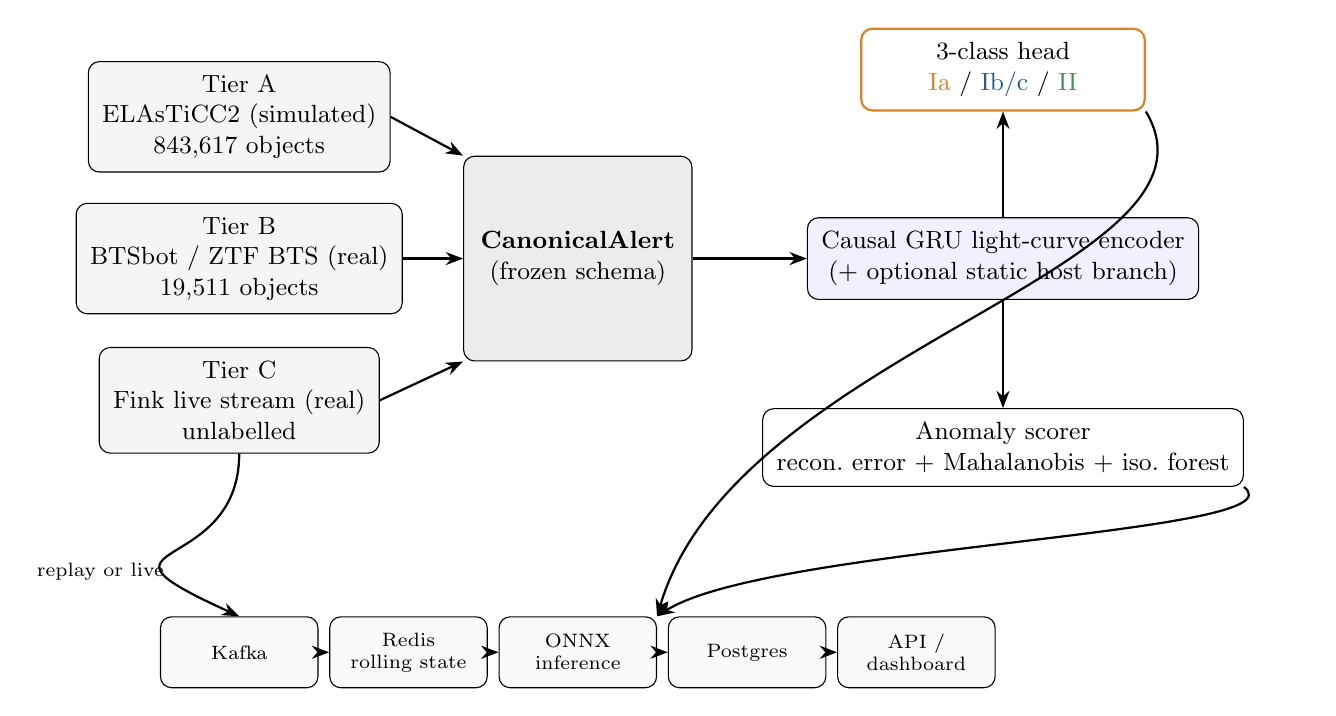
\begin{tikzpicture}[
  font=\small,
  box/.style={draw, rounded corners, align=center, minimum height=0.9cm, inner sep=5pt},
  tier/.style={box, minimum width=3.4cm, fill=gray!8},
  funnel/.style={draw, rounded corners, minimum width=2.9cm, minimum height=2.6cm, align=center, fill=gray!15},
  enc/.style={box, minimum width=4.8cm, fill=blue!6},
  head/.style={box, minimum width=3.6cm},
  serve/.style={box, minimum width=2.0cm, fill=gray!5, font=\scriptsize},
  arr/.style={-{Stealth[length=2.2mm]}, thick},
  >=Stealth,
]

% --- data tiers (left column) ---
\node[tier] (tiera) at (0, 5.4) {Tier A\\ELAsTiCC2 (simulated)\\843{,}617 objects};
\node[tier] (tierb) at (0, 3.6) {Tier B\\BTSbot / ZTF BTS (real)\\19{,}511 objects};
\node[tier] (tierc) at (0, 1.8) {Tier C\\Fink live stream (real)\\unlabelled};

% --- canonical schema funnel ---
\node[funnel] (schema) at (4.3, 3.6) {\textbf{CanonicalAlert}\\(frozen schema)};

\draw[arr] (tiera.east) -- (schema.north west);
\draw[arr] (tierb.east) -- (schema.west);
\draw[arr] (tierc.east) -- (schema.south west);

% --- encoder ---
\node[enc] (encoder) at (9.7, 3.6) {Causal GRU light-curve encoder\\(+ optional static host branch)};
\draw[arr] (schema) -- (encoder);

% --- heads ---
\node[head, draw=classIa, thick] (clshead) at (9.7, 6.0) {3-class head\\\textcolor{classIa}{Ia} / \textcolor{classIbc}{Ib/c} / \textcolor{classII}{II}};
\node[head] (anomhead) at (9.7, 1.2) {Anomaly scorer\\recon.\ error + Mahalanobis + iso.\ forest};
\draw[arr] (encoder.north) -- (clshead.south);
\draw[arr] (encoder.south) -- (anomhead.north);

% --- serving path (bottom row) ---
\node[serve] (kafka) at (0.0, -1.4) {Kafka};
\node[serve] (redis) at (2.15, -1.4) {Redis\\rolling state};
\node[serve] (onnx) at (4.3, -1.4) {ONNX\\inference};
\node[serve] (pg) at (6.45, -1.4) {Postgres};
\node[serve] (api) at (8.6, -1.4) {API /\\dashboard};

\draw[arr] (kafka) -- (redis);
\draw[arr] (redis) -- (onnx);
\draw[arr] (onnx) -- (pg);
\draw[arr] (pg) -- (api);

\draw[arr] (tierc.south) .. controls +(0,-1.6) and +(-2.2,1.0) .. (kafka.north)
  node[midway, below left, font=\scriptsize] {replay or live};
\draw[arr] (clshead.south east) .. controls +(1.2,-2.0) and +(1.0,3.4) .. (onnx.north east);
\draw[arr] (anomhead.south east) .. controls +(0.8,-0.6) and +(1.4,0.9) .. (onnx.north east);

\end{tikzpicture}

% from paper/sections/methodology.tex.
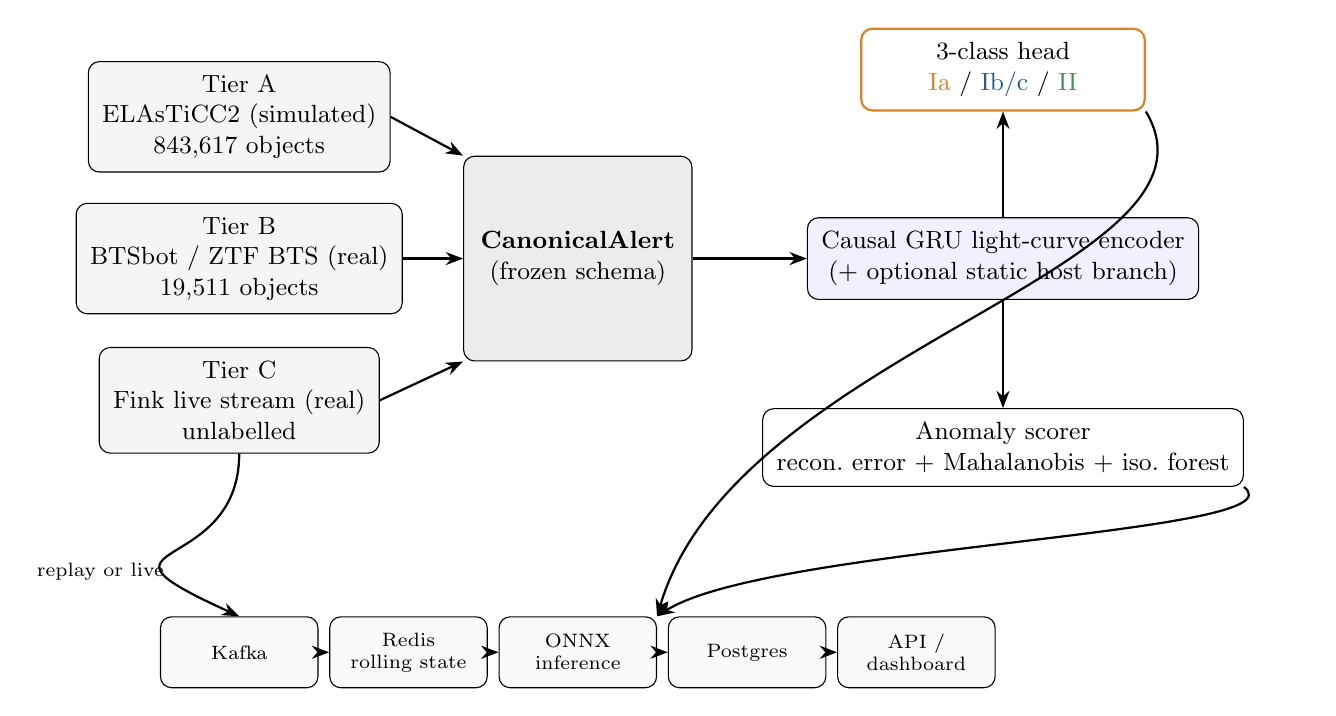
\begin{tikzpicture}[
  font=\small,
  box/.style={draw, rounded corners, align=center, minimum height=0.9cm, inner sep=5pt},
  tier/.style={box, minimum width=3.4cm, fill=gray!8},
  funnel/.style={draw, rounded corners, minimum width=2.9cm, minimum height=2.6cm, align=center, fill=gray!15},
  enc/.style={box, minimum width=4.8cm, fill=blue!6},
  head/.style={box, minimum width=3.6cm},
  serve/.style={box, minimum width=2.0cm, fill=gray!5, font=\scriptsize},
  arr/.style={-{Stealth[length=2.2mm]}, thick},
  >=Stealth,
]

% --- data tiers (left column) ---
\node[tier] (tiera) at (0, 5.4) {Tier A\\ELAsTiCC2 (simulated)\\843{,}617 objects};
\node[tier] (tierb) at (0, 3.6) {Tier B\\BTSbot / ZTF BTS (real)\\19{,}511 objects};
\node[tier] (tierc) at (0, 1.8) {Tier C\\Fink live stream (real)\\unlabelled};

% --- canonical schema funnel ---
\node[funnel] (schema) at (4.3, 3.6) {\textbf{CanonicalAlert}\\(frozen schema)};

\draw[arr] (tiera.east) -- (schema.north west);
\draw[arr] (tierb.east) -- (schema.west);
\draw[arr] (tierc.east) -- (schema.south west);

% --- encoder ---
\node[enc] (encoder) at (9.7, 3.6) {Causal GRU light-curve encoder\\(+ optional static host branch)};
\draw[arr] (schema) -- (encoder);

% --- heads ---
\node[head, draw=classIa, thick] (clshead) at (9.7, 6.0) {3-class head\\\textcolor{classIa}{Ia} / \textcolor{classIbc}{Ib/c} / \textcolor{classII}{II}};
\node[head] (anomhead) at (9.7, 1.2) {Anomaly scorer\\recon.\ error + Mahalanobis + iso.\ forest};
\draw[arr] (encoder.north) -- (clshead.south);
\draw[arr] (encoder.south) -- (anomhead.north);

% --- serving path (bottom row) ---
\node[serve] (kafka) at (0.0, -1.4) {Kafka};
\node[serve] (redis) at (2.15, -1.4) {Redis\\rolling state};
\node[serve] (onnx) at (4.3, -1.4) {ONNX\\inference};
\node[serve] (pg) at (6.45, -1.4) {Postgres};
\node[serve] (api) at (8.6, -1.4) {API /\\dashboard};

\draw[arr] (kafka) -- (redis);
\draw[arr] (redis) -- (onnx);
\draw[arr] (onnx) -- (pg);
\draw[arr] (pg) -- (api);

\draw[arr] (tierc.south) .. controls +(0,-1.6) and +(-2.2,1.0) .. (kafka.north)
  node[midway, below left, font=\scriptsize] {replay or live};
\draw[arr] (clshead.south east) .. controls +(1.2,-2.0) and +(1.0,3.4) .. (onnx.north east);
\draw[arr] (anomhead.south east) .. controls +(0.8,-0.6) and +(1.4,0.9) .. (onnx.north east);

\end{tikzpicture}
}
\end{center}

\bigskip
\noindent\textit{Pipeline architecture.} Three data tiers (simulated
ELAsTiCC2 for pretraining, real ZTF/BTSbot for fine-tuning, live Fink for
serving) convert into one canonical alert schema, which every downstream
stage consumes identically regardless of source. A shared causal GRU
light-curve encoder (optionally fused with a static host-context branch)
feeds both the flat 3-class classification head and a separate
anomaly-scoring branch. The serving path (Kafka $\to$ Redis rolling state
$\to$ ONNX inference $\to$ Postgres $\to$ API) is the same consumer code
whether its producer is an archived-data replay or the live Fink stream.
This same diagram recurs as Figure~\ref{fig:pipeline} in
Chapter~\ref{sec:methodology-chapter}, where each stage is discussed in
detail.

\clearpage

\section*{Acknowledgements}
\addcontentsline{toc}{section}{Acknowledgements}

This work was completed as the final deliverable for the Summer School of
Astronomy and Astrophysics, organised by the Indian Space School in
collaboration with the Propagation Institute of Space and Technology
(PIST); we thank the programme for the brief and the opportunity. We thank
the LSST Dark Energy Science Collaboration for the public ELAsTiCC2
training-sample release; the Zwicky Transient Facility Bright Transient
Survey and the BTSbot authors for the public metadata release and the BTS
Sample Explorer; the Fink broker team for public, credentialled access to
live ZTF and LSST alert streams; and the SNAD team for the
\texttt{coniferest} anomaly-detection package.

\clearpage

\tableofcontents
\clearpage
\listoffigures
\clearpage
\listoftables
\clearpage

% ==================== Main matter (arabic numerals) ====================
\pagenumbering{arabic}
\setcounter{page}{1}

\section{Introduction, Literature Survey, Methodology, Objectives}

\subsection{Introduction}
\label{sec:introduction}

A supernova is the catastrophic, once-per-object brightening of a star
(or stellar remnant) at the end point of its evolution. For a period of
days to months it can rival or exceed the integrated brightness of its
entire host galaxy, which is what makes supernovae visible across cosmological
distances and useful as tracers of the universe's structure and expansion.
Astronomers group observed supernovae by \emph{spectroscopic type}: what
absorption and emission features appear when the transient's light is
dispersed through a spectrograph. This report is concerned with three of
those types, and with a fourth category -- ``none of the above'' -- that a
real alert stream inevitably also produces.

\paragraph{Two unrelated physical channels, one shared naming scheme.}
Type Ia supernovae arise from the thermonuclear disruption of a carbon-oxygen
white dwarf, either through mass accretion from a companion star past a
critical threshold or through the merger of two white dwarfs. The explosion
consumes the star with no hydrogen involved at any stage, which is why a Ia
spectrum shows no hydrogen lines. Type Ib/c and Type II supernovae, by
contrast, are both \emph{core-collapse} events: a massive star ($\gtrsim
8\,M_\odot$) exhausts its nuclear fuel, its iron core can no longer support
itself against gravity, and the resulting collapse (typically to a neutron
star) drives a shock that unbinds the star's outer layers. Type II
supernovae still have their hydrogen envelope at the moment of collapse;
Type Ib and Ic supernovae have already lost it (and, for Ic, their helium
layer too) to strong stellar winds or to a binary companion. It is worth
stating plainly, because the shared Roman-numeral naming scheme actively
obscures it: \emph{Type Ia is not physically related to Type Ib or Ic}. The
``I'' in each name refers only to the historical absence of hydrogen lines
in the discovery-era spectroscopic classification scheme
\citep{filippenko1997}, not to a shared progenitor or explosion mechanism.
Type Ib and Ic are two flavours of the same core-collapse channel as Type
II; Type Ia is a different channel entirely. This project follows
convention (and its own taxonomy, Section~\ref{sec:data}) in merging Ib and
Ic into one target class, since distinguishing a stripped-envelope
supernova that has lost its hydrogen from one that has lost its helium as
well requires spectroscopy this pipeline does not have.

\paragraph{Why Type Ia matters beyond stellar physics.}
Because a Type Ia explosion detonates a white dwarf at (or close to) a
common physical trigger mass, the resulting explosions are photometrically
similar to one another: their peak absolute brightness is
\emph{standardisable} through empirical relations between peak luminosity,
light-curve decline rate, and colour. That standardisability is what turns
a Type Ia supernova into a ``standard candle'' -- an object whose true
brightness can be inferred well enough from its light curve alone that
comparing it to its \emph{observed} brightness yields a distance. Type Ia
supernovae were the tool used to discover the accelerating expansion of the
universe, and they remain a primary distance-ladder rung today. Recovering
Ia identity from photometry alone, quickly, is therefore not merely a
pattern-recognition exercise: it is a prerequisite for using a given object
cosmologically at all.

\paragraph{Spectroscopy is definitive; photometry is what scales.}
A spectrum directly measures the physics -- the elements present, their
ionisation state, the ejecta's expansion velocity -- and is the only fully
reliable way to assign a supernova's type. It is also expensive: it requires
a sufficiently large telescope, a spectrograph, and dedicated observing time
allocated to one object at a time. What a wide-field synoptic survey
produces automatically, for every object, every time it is observed, is a
\emph{light curve}: a sequence of calibrated flux measurements at a handful
of timestamps and wavelength filters (``bands''). The central question this
project asks is how much of the spectroscopic answer -- Ia, Ib/c, or II --
can be recovered from a light curve's shape alone: how fast it rises, how
it declines, whether it plateaus, all without ever taking a spectrum. Doing
this \emph{early}, before the light curve has finished playing out, is the
useful case in practice: a system that can say ``point a spectrograph at
this one'' while the transient is still spectroscopically interesting is
worth far more than one that can only classify a supernova after it has
faded.

\paragraph{The scale problem.}
The Zwicky Transient Facility (ZTF) already produces alert volumes that
strain manual and even semi-automated triage
\citep{bellm2019ztf}. The Vera C.\ Rubin Observatory's Legacy Survey of
Space and Time (LSST), whose main ten-year survey began operations on 30
June 2026, is designed to generate on the order of $10^7$ transient and
variable-source alerts per night at full operational cadence
\citep{ivezic2019lsst} -- a volume no spectroscopic follow-up programme,
however well resourced, can classify object by object. Automated,
photometry-only triage is therefore not an optional convenience for the
LSST era; it is the only mechanism by which a human-in-the-loop follow-up
programme can be pointed at the right handful of objects out of millions.
This report describes one such triage system, built and measured against
both simulated LSST-like data and real ZTF data, and served, briefly, over
a live alert stream from both surveys.

\subsection{Motive and Objectives}
\label{sec:objectives}

The programme brief, as set by the Summer School of Astronomy and
Astrophysics, asked for a multi-survey, multimodal pipeline that classifies
transient alerts into supernova subtypes and flags objects that fit none of
them, pretrained on simulated data, fine-tuned on real spectroscopically
labelled data, served over a live alert stream, and refined by a
human-in-the-loop anomaly review process. From that brief, seven concrete,
individually testable objectives were set at the start of the project:

\begin{enumerate}
  \item Build a single canonical data schema and one reader per data source
    (simulated ELAsTiCC2, real ZTF/BTSbot, live Fink) that converts each
    source into it, so that a model trained on one source can be evaluated
    on another without a source-specific code path.
  \item Train a causal light-curve classifier on simulated data alone and
    establish its ceiling performance and failure modes before any real
    data is introduced.
  \item Fine-tune that classifier on real, spectroscopically labelled data
    and \emph{measure} the resulting sim-to-real accuracy gap, rather than
    assume fine-tuning succeeds.
  \item Build a separate anomaly-detection branch capable of ranking alerts
    that do not resemble any of the three target classes, and evaluate it
    against both a simulated held-out anomaly population and a real one.
  \item Serve the trained models over a Kafka-based pipeline, first in
    replay mode against archived data and then, unmodified, against a live
    alert stream from at least one real broker.
  \item Validate every stage against pre-registered acceptance criteria
    (Section~\ref{sec:methodology}'s four gates) defined \emph{before} the
    results they judge, rather than criteria chosen after the fact to match
    whatever result was obtained.
  \item Produce a results and monitoring interface that makes every reported
    number traceable to the artifact that produced it.
\end{enumerate}

Sections~\ref{sec:data}--\ref{sec:results} report the outcome of each
objective in turn; Section~\ref{sec:discussion} discusses which were fully
met, which were only partially met, and why.


\subsection{Literature Survey}
\label{sec:literature}

\paragraph{Recurrent networks on raw light curves.}
\citet{charnock2017} were among the first to show that a recurrent neural
network fed raw, un-engineered light-curve photometry directly could
classify supernova types competitively with feature-engineering pipelines,
on simulated Dark Energy Survey-like data -- establishing that a sequence
model need not first be handed hand-built summary statistics (rise time,
colour at peak, and so on) to find useful structure in a light curve.
\citet{muthukrishna2019rapid} extended this to \emph{early}, time-resolved
classification with RAPID, a Gated Recurrent Unit (GRU) architecture that
emits a classification at every observed timestep rather than only at the
end of a light curve, across 12 transient classes; this per-timestep
prediction convention, and the resulting practice of reporting accuracy as
a function of time since first detection rather than as one end-of-light-
curve number, is used throughout the present work (Section~\ref{sec:analysis}).
\citet{moller2020supernnova} (SuperNNova) placed a Bayesian recurrent
architecture in this same family, adding calibrated uncertainty estimates
and a systematic comparison against feature-based random-forest baselines,
run at ZTF and LSST alert-stream scale.

\paragraph{Data challenges.}
\citet{kessler2019plasticc} designed and described PLAsTiCC, the Photometric
LSST Astronomical Time-series Classification Challenge: a large, publicly
released simulated dataset spanning many transient and variable-source
classes, intended to let classification methods be compared on a common,
labelled corpus before real LSST data existed. ELAsTiCC2 \citep{elasticc2},
the LSST Dark Energy Science Collaboration's Extended LSST Astronomical
Time-series Classification Challenge and this project's own Tier A
simulated corpus (Section~\ref{sec:data}), supersedes PLAsTiCC with an
updated simulation
pipeline, revised class definitions, and -- the property this project
depends on most directly -- deliberately \emph{non}-representative class
proportions relative to the real sky rate, so that a classifier trained on
it must be evaluated with that mismatch in mind rather than assumed to
inherit a realistic prior (Section~\ref{sec:data}).

\paragraph{Current state of the art.}
\citet{cabreravives2024atat} report ATAT, a pair of transformer encoders
(one over the light curve, one over tabular host/metadata features) fused
before a classification head, reaching a macro-F1 of $82.9 \pm 0.4$ across
20 ELAsTiCC classes -- the strongest published number on this class of
problem to date, and the anchor this project's own, considerably smaller
3-class macro-F1 figures should be read against, not compared to directly
(Section~\ref{sec:results}). \citet{shah2025oracle} (ORACLE) instead build
a GRU-based hierarchical classifier trained with a hierarchical
cross-entropy loss and host-galaxy context, explicitly targeting the same
graceful-degradation property (a correct ``supernova-like'' call even when
the fine-grained subtype call is wrong) that this project's own hierarchical
loss experiment tests and does not, in the end, adopt
(Section~\ref{sec:methodology}). A causal-transformer architecture for this
same task is described in \citet{atcat2025}, reporting 71.8\% light-curve-only
and 89.8\% light-curve-plus-metadata F1 on their own evaluation. Fine-grained
supernova subtyping is consistently reported, across this literature, as a
harder discrimination axis than the coarser transient-vs-non-transient call
-- consistent with this project's own recorded expectation that the Ib/c
class in particular should be, and is, the hardest of the three target
classes to recover cleanly.

\paragraph{Anomaly detection over alert streams.}
\citet{malanchev2021} ran an unsupervised anomaly detector (isolation-forest-
based) over ZTF's third public data release and reported that of the
highest-ranked, most anomalous objects a human inspected, 68\% were
artifacts of imperfect image subtraction rather than genuine unusual
transients -- the published anchor this project's own Gate D (deferred, not
passed -- Section~\ref{sec:results}) was designed to be checked against.
\citet{villar2021vraenn} (VRAENN) instead trained a variational recurrent
autoencoder for the same live-anomaly-detection task, an architecture whose
reconstruction-error principle is close in spirit to the decoder component
of this project's own three-part anomaly score
(Section~\ref{sec:methodology}). \texttt{coniferest} \citep{coniferest}, the
isolation-forest and active-learning package used here for one of the three
anomaly components, is developed and maintained by the SNAD (SNAD Anomaly
Detection) team; the production Fink broker's own anomaly-ranking module,
described in \citet{moller2021fink}, is built on the same package.

\paragraph{Real data and brokers.}
The Zwicky Transient Facility Bright Transient Survey (BTS,
\citealp{fremling2020bts,perley2020bts}) is the source of this project's
real, spectroscopically labelled fine-tuning data (Tier B). BTSbot
\citep{rehemtulla2024btsbot} is a real-bogus and bright-transient-vs-reject
triage classifier trained on the same BTS alert stream; this project reuses
its public metadata release as the raw Tier B corpus (Section~\ref{sec:data})
but not its own triage labels, which answer a different question (``is this
a real, bright transient at all'') from the one this project trains on
(``which of Ia/Ib-c/II is it''). ALeRCE \citep{forster2021alerce} and Fink
\citep{moller2021fink} are both production alert brokers that ingest ZTF
(and, for Fink, LSST) alert streams and run their own classification and
anomaly-ranking pipelines in real time; Fink is the broker this project's
own serving layer (Section~\ref{sec:methodology}) actually connects to for
live Tier C data.

\paragraph{Transfer learning.}
\citet{guptamuthukrishna2025} report that pretraining a transient classifier
on simulated data and fine-tuning on a comparatively small real labelled
ZTF set reduces the amount of real labelled data needed by about 75\%
relative to training on real data alone, and that a model pretrained on
ZTF reaches 94\% of a from-scratch baseline's performance on simulated LSST
data using only 30\% as much LSST training data -- the same sim-to-real
transfer strategy this project's own Tier A~$\to$~Tier B pipeline follows
(in the opposite direction, LSST-like simulation to real ZTF), and the same
comparison (zero-shot Tier-A-only performance versus fine-tuned performance
on Tier B) this project measures directly in Section~\ref{sec:results}.

\paragraph{Loss design.}
\citet{villar2023whxe} propose weighted hierarchical cross-entropy (WHXE): a
loss that predicts at every level of a class taxonomy tree, not only at the
leaf, and weights a mistake by how far apart the true and predicted classes
sit in that tree -- confusing two supernova subtypes should cost less than
confusing a supernova with a non-supernova. This project implements WHXE
essentially as published, encounters and resolves a real ambiguity in the
paper's own depth-indexing convention, and reports a controlled, one-run
comparison against a flat classification head that does not favour WHXE on
this project's own single-branch dataset (Section~\ref{sec:methodology});
this is stated as a property of the data available at the time of the
comparison, not as a criticism of the loss itself.

\paragraph{Surveys.}
\citet{bellm2019ztf} describe ZTF's system design, cadence, and early
performance; \citet{ivezic2019lsst} describe LSST's science drivers,
reference design, and anticipated data products, including the alert-volume
figures cited in Section~\ref{sec:introduction}.

\paragraph{Taxonomy.}
\citet{filippenko1997} is the standard review of the spectroscopic
classification scheme this entire field, and this project's own taxonomy
(Section~\ref{sec:data}), is built on.

\paragraph{Where this work sits.}
None of the architectural components used here are novel: a causal GRU
light-curve encoder, a reconstruction-error/Mahalanobis/isolation-forest
anomaly ensemble, and a Kafka-based serving layer are all established
techniques, individually published elsewhere in the works cited above. What
this report adds is not a new architecture but a measured, audited account
of what happens when a comparatively standard pipeline of this kind is
actually built end to end on a strict timeline: a quantified sim-to-real
transfer gap and transfer gain (Section~\ref{sec:results}); a documented
account of where the train-time and serve-time data distributions silently
diverge and what that costs (Section~\ref{sec:analysis}); a measured,
non-obvious failure mode in the anomaly ensemble under domain shift
(Section~\ref{sec:results}); and end-to-end serving and live-ingestion
results, run against real ZTF and LSST alert traffic, that are not published
elsewhere for a pipeline of this specific shape. Understating this
contribution is the safer error to make, and is made deliberately.


\chapter{Methodology, Data \& Observations}
\label{sec:methodology-chapter}

\section{Methodology}
\label{sec:methodology}

This section states the design principles adopted \emph{before} any model
was trained or any result existed, the resulting architecture, and the
validation protocol used to judge every result reported in
Section~\ref{sec:results}. Table~\ref{tab:decisionlog} at the end of this
section is a decision log: for each major design choice, the alternatives
considered, the choice made, and the evidence that settled it. Most write-ups
of a pipeline like this present only the final configuration; the
alternatives that were rejected, and why, are at least as informative.

\subsection{Design principles}

\paragraph{Wavelength conditioning, not band identity.}
ZTF alerts carry three photometric filters; LSST alerts carry six
(Table~\ref{tab:lameff}). If a model's input encoded ``filter index 2,''
ZTF's second filter and LSST's second filter would be unrelated integers
occupying unrelated positions in the model's input space, and nothing
learned from simulated LSST photometry (Tier A) would transfer to real ZTF
photometry (Tier B) at all. Instead, every observation in this pipeline
carries its filter's actual \emph{effective wavelength}, a continuous
physical quantity, linearly mapped into $[-1, 1]$
(Section~\ref{sec:analysis}). ZTF's $r$ band (633.9\,nm) and LSST's $r$ band
(622.2\,nm) land near each other in the model's input space automatically,
because they are physically similar wavelengths, not because any code
special-cases ``these are both called $r$.'' This single decision is what
makes ``pretrain on simulated LSST photometry, fine-tune on real ZTF
photometry'' a coherent strategy rather than two unrelated models sharing a
name.

\begin{table}[htb]
\centering
\caption{Filter effective wavelengths used for wavelength conditioning
(Section~\ref{sec:methodology}). LSST's six bands and ZTF's three are
mapped into the same continuous space; no band index is ever used as a
model input.}
\label{tab:lameff}
\begin{tabular}{ccccc}
\toprule
\multicolumn{2}{c}{LSST} & & \multicolumn{2}{c}{ZTF} \\
Band & $\lambda_\mathrm{eff}$ (nm) & & Band & $\lambda_\mathrm{eff}$ (nm) \\
\midrule
$u$ & 368.6 & & $g$ & 472.3 \\
$g$ & 480.3 & & $r$ & 633.9 \\
$r$ & 622.2 & & $i$ & 788.6 \\
$i$ & 754.5 & & & \\
$z$ & 869.1 & & & \\
$y$ & 971.0 & & & \\
\bottomrule
\end{tabular}
\end{table}

\paragraph{Causal models only.}
Every recurrent layer in this pipeline runs in a single direction only
(\texttt{bidirectional=False} throughout), with no attention mechanism
that could attend to a future timestep. A bidirectional model evaluated
offline, where
every object's complete light curve already exists in the training set,
would silently learn to use information from an object's future relative to
whatever point it is nominally classifying at -- on day 3 of a real alert
stream, day 60 has not happened yet. Such a model scores well offline and is
meaningless in production, and the failure would not be visible in any
ordinary train/test split, since both sides of that split share the same
non-causal leakage. This is treated as an absolute architectural constraint,
not a tunable hyperparameter, and is enforced by a dedicated unit test that
truncates a real input sequence at a timestep $t$ and asserts the model's
prediction at $t$ is bit-identical whether or not timesteps after $t$ are
present in the input tensor at all (Table~\ref{tab:gates}, Gate B).

\paragraph{A frozen evaluation harness.}
The canonical data schema and the evaluation metrics code were written and
frozen before any model existed, and were never modified afterward except
by one documented, additive amendment (below). The reasoning is that a
metric implementation that can still be edited is a metric that will,
eventually, be adjusted -- consciously or not -- to make a disappointing
result look better, and the resulting number would be unfalsifiable: there
would be no way to tell ``the model improved'' from ``the yardstick moved''
after the fact. The one amendment made to the frozen harness after Day~1
was the addition of ROC-AUC (Ia-vs-rest) as a new metric, once the project's
own literature anchors (Section~\ref{sec:literature}) turned out to name a
metric that did not yet exist anywhere in the harness. The amendment added a
new function and the minimal wiring to carry its output through the existing
report structures, touched no existing function's computed output, and was
verified independently (a new value on an existing checkpoint, not a
retroactive recomputation of an existing reported number). An amendment of
this kind -- additive, independently verified, motivated by a real gap
rather than a disappointing result -- is judged preferable to a blanket
no-changes rule that would otherwise have blocked a metric the project's
own anchors required.

\paragraph{Flux, never magnitude.}
Difference-image photometry -- subtracting a reference template from a new
science exposure -- routinely produces negative flux values on noisy,
faint, non-detections. Those points are concentrated in exactly the early,
pre-peak regime this project's early-classification goal cares about most.
A magnitude is a logarithm of flux and cannot represent a negative value at
all; any reader that converts to magnitude before this pipeline sees the
data has already silently discarded some of the most informative early-time
points. Every reader in this pipeline therefore emits flux, on one shared
zeropoint (Section~\ref{sec:data}), and only ever converts to magnitude for
plotting.

\paragraph{A canonical alert schema as the single conversion target.}
Every data source -- simulated ELAsTiCC2, real ZTF/BTSbot, live Fink -- is
converted into one shared \texttt{CanonicalAlert} record before any model
or evaluation code ever touches it (Table~\ref{tab:schema}). This is what
makes ``pretrain on one source, fine-tune on another, serve a third''
possible without a source-specific branch anywhere downstream of the reader
layer.

\begin{table}[htb]
\centering
\caption{The canonical alert schema (\texttt{src/schema.py}, frozen after
Day 1--2 of the project). Every reader converts its source into this record;
no downstream code depends on which survey an alert came from.}
\label{tab:schema}
\begin{tabular}{L{2.6cm}L{10.9cm}}
\toprule
Field & Meaning \\
\midrule
\texttt{object\_id} & Survey-native identifier \\
\texttt{survey} & ZTF / LSST / ELAsTiCC \\
\texttt{observations} & List of (mjd, $\lambda_\mathrm{eff}$, flux, flux\_err, is\_detection), sorted ascending by mjd \\
\texttt{static} & Host photo-$z$, offset, ellipticity, host magnitude, MW $E(B\!-\!V)$, galactic latitude, real-bogus score \\
\texttt{cutouts} & $(3,63,63)$ science/reference/difference postage stamps, or \texttt{None} \\
\texttt{class\_id} & ELAsTiCC2 taxonomy id (Table~\ref{tab:taxonomy}), or \texttt{None} if unlabelled \\
\bottomrule
\end{tabular}
\end{table}

\subsection{Figure 1: pipeline architecture}

Figure~\ref{fig:pipeline} is the anchor figure for this report: the three
data tiers on the left, the canonical schema as the single conversion
funnel every tier passes through, the shared light-curve encoder feeding
both the classification head and the anomaly scorer, and the serving path
from a live alert stream through to a results interface.

\begin{figure}[htb]
\centering
\resizebox{\linewidth}{!}{% Figure 1: pipeline architecture. Included via % Figure 1: pipeline architecture. Included via \input{figures/fig1_pipeline}
% from paper/sections/methodology.tex.
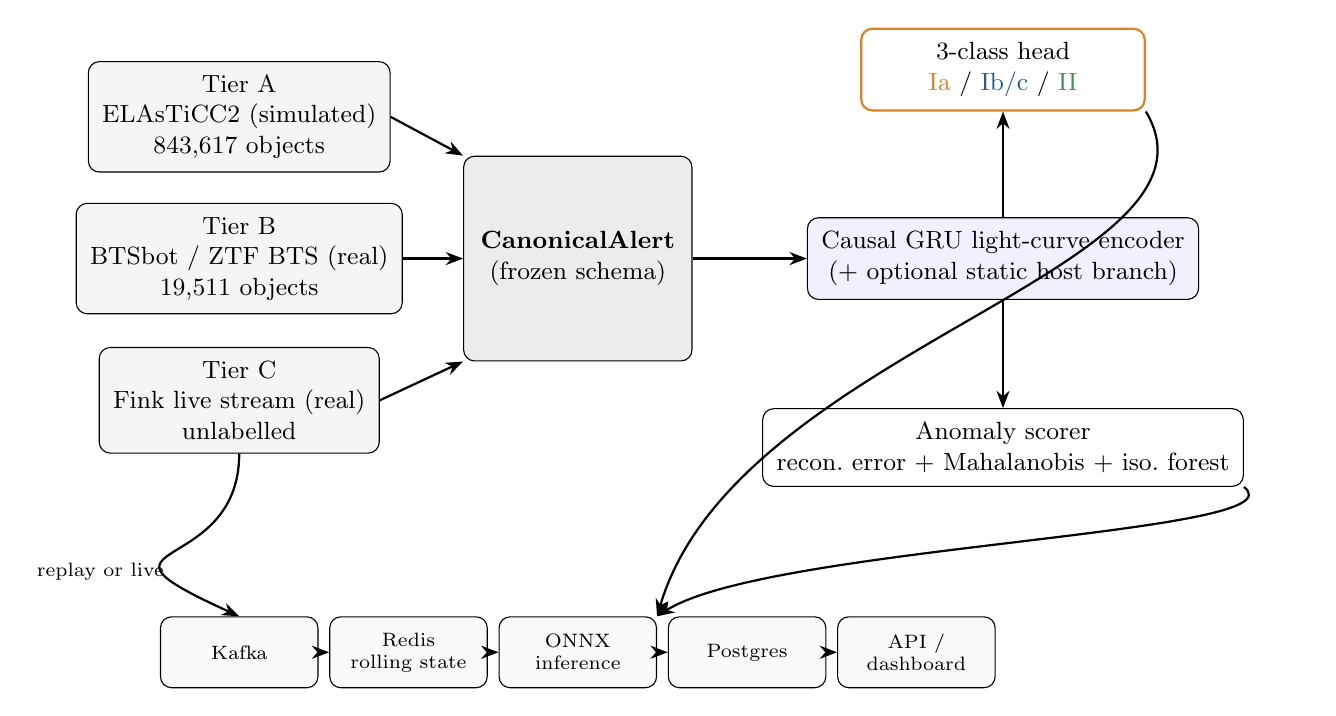
\begin{tikzpicture}[
  font=\small,
  box/.style={draw, rounded corners, align=center, minimum height=0.9cm, inner sep=5pt},
  tier/.style={box, minimum width=3.4cm, fill=gray!8},
  funnel/.style={draw, rounded corners, minimum width=2.9cm, minimum height=2.6cm, align=center, fill=gray!15},
  enc/.style={box, minimum width=4.8cm, fill=blue!6},
  head/.style={box, minimum width=3.6cm},
  serve/.style={box, minimum width=2.0cm, fill=gray!5, font=\scriptsize},
  arr/.style={-{Stealth[length=2.2mm]}, thick},
  >=Stealth,
]

% --- data tiers (left column) ---
\node[tier] (tiera) at (0, 5.4) {Tier A\\ELAsTiCC2 (simulated)\\843{,}617 objects};
\node[tier] (tierb) at (0, 3.6) {Tier B\\BTSbot / ZTF BTS (real)\\19{,}511 objects};
\node[tier] (tierc) at (0, 1.8) {Tier C\\Fink live stream (real)\\unlabelled};

% --- canonical schema funnel ---
\node[funnel] (schema) at (4.3, 3.6) {\textbf{CanonicalAlert}\\(frozen schema)};

\draw[arr] (tiera.east) -- (schema.north west);
\draw[arr] (tierb.east) -- (schema.west);
\draw[arr] (tierc.east) -- (schema.south west);

% --- encoder ---
\node[enc] (encoder) at (9.7, 3.6) {Causal GRU light-curve encoder\\(+ optional static host branch)};
\draw[arr] (schema) -- (encoder);

% --- heads ---
\node[head, draw=classIa, thick] (clshead) at (9.7, 6.0) {3-class head\\\textcolor{classIa}{Ia} / \textcolor{classIbc}{Ib/c} / \textcolor{classII}{II}};
\node[head] (anomhead) at (9.7, 1.2) {Anomaly scorer\\recon.\ error + Mahalanobis + iso.\ forest};
\draw[arr] (encoder.north) -- (clshead.south);
\draw[arr] (encoder.south) -- (anomhead.north);

% --- serving path (bottom row) ---
\node[serve] (kafka) at (0.0, -1.4) {Kafka};
\node[serve] (redis) at (2.15, -1.4) {Redis\\rolling state};
\node[serve] (onnx) at (4.3, -1.4) {ONNX\\inference};
\node[serve] (pg) at (6.45, -1.4) {Postgres};
\node[serve] (api) at (8.6, -1.4) {API /\\dashboard};

\draw[arr] (kafka) -- (redis);
\draw[arr] (redis) -- (onnx);
\draw[arr] (onnx) -- (pg);
\draw[arr] (pg) -- (api);

\draw[arr] (tierc.south) .. controls +(0,-1.6) and +(-2.2,1.0) .. (kafka.north)
  node[midway, below left, font=\scriptsize] {replay or live};
\draw[arr] (clshead.south east) .. controls +(1.2,-2.0) and +(1.0,3.4) .. (onnx.north east);
\draw[arr] (anomhead.south east) .. controls +(0.8,-0.6) and +(1.4,0.9) .. (onnx.north east);

\end{tikzpicture}

% from paper/sections/methodology.tex.
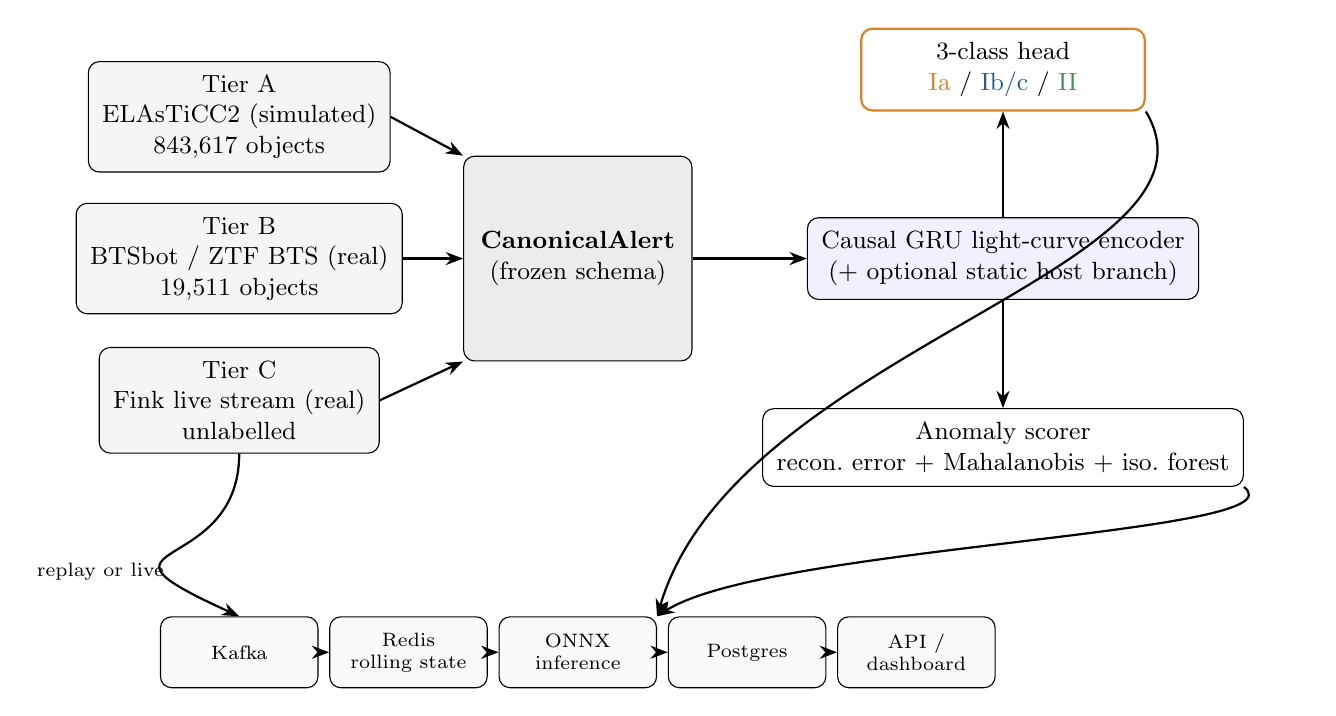
\begin{tikzpicture}[
  font=\small,
  box/.style={draw, rounded corners, align=center, minimum height=0.9cm, inner sep=5pt},
  tier/.style={box, minimum width=3.4cm, fill=gray!8},
  funnel/.style={draw, rounded corners, minimum width=2.9cm, minimum height=2.6cm, align=center, fill=gray!15},
  enc/.style={box, minimum width=4.8cm, fill=blue!6},
  head/.style={box, minimum width=3.6cm},
  serve/.style={box, minimum width=2.0cm, fill=gray!5, font=\scriptsize},
  arr/.style={-{Stealth[length=2.2mm]}, thick},
  >=Stealth,
]

% --- data tiers (left column) ---
\node[tier] (tiera) at (0, 5.4) {Tier A\\ELAsTiCC2 (simulated)\\843{,}617 objects};
\node[tier] (tierb) at (0, 3.6) {Tier B\\BTSbot / ZTF BTS (real)\\19{,}511 objects};
\node[tier] (tierc) at (0, 1.8) {Tier C\\Fink live stream (real)\\unlabelled};

% --- canonical schema funnel ---
\node[funnel] (schema) at (4.3, 3.6) {\textbf{CanonicalAlert}\\(frozen schema)};

\draw[arr] (tiera.east) -- (schema.north west);
\draw[arr] (tierb.east) -- (schema.west);
\draw[arr] (tierc.east) -- (schema.south west);

% --- encoder ---
\node[enc] (encoder) at (9.7, 3.6) {Causal GRU light-curve encoder\\(+ optional static host branch)};
\draw[arr] (schema) -- (encoder);

% --- heads ---
\node[head, draw=classIa, thick] (clshead) at (9.7, 6.0) {3-class head\\\textcolor{classIa}{Ia} / \textcolor{classIbc}{Ib/c} / \textcolor{classII}{II}};
\node[head] (anomhead) at (9.7, 1.2) {Anomaly scorer\\recon.\ error + Mahalanobis + iso.\ forest};
\draw[arr] (encoder.north) -- (clshead.south);
\draw[arr] (encoder.south) -- (anomhead.north);

% --- serving path (bottom row) ---
\node[serve] (kafka) at (0.0, -1.4) {Kafka};
\node[serve] (redis) at (2.15, -1.4) {Redis\\rolling state};
\node[serve] (onnx) at (4.3, -1.4) {ONNX\\inference};
\node[serve] (pg) at (6.45, -1.4) {Postgres};
\node[serve] (api) at (8.6, -1.4) {API /\\dashboard};

\draw[arr] (kafka) -- (redis);
\draw[arr] (redis) -- (onnx);
\draw[arr] (onnx) -- (pg);
\draw[arr] (pg) -- (api);

\draw[arr] (tierc.south) .. controls +(0,-1.6) and +(-2.2,1.0) .. (kafka.north)
  node[midway, below left, font=\scriptsize] {replay or live};
\draw[arr] (clshead.south east) .. controls +(1.2,-2.0) and +(1.0,3.4) .. (onnx.north east);
\draw[arr] (anomhead.south east) .. controls +(0.8,-0.6) and +(1.4,0.9) .. (onnx.north east);

\end{tikzpicture}
}
\caption{Pipeline architecture. Three data tiers (simulated ELAsTiCC2 for
pretraining, real ZTF/BTSbot for fine-tuning, live Fink for serving) convert
into one canonical alert schema, which every downstream stage consumes
identically regardless of source. A shared causal GRU light-curve encoder
(optionally fused with a static host-context branch) feeds both the flat
3-class classification head and a separate anomaly-scoring branch. The
serving path (Kafka $\to$ Redis rolling state $\to$ ONNX inference $\to$
Postgres $\to$ API) is the same consumer code whether its producer is an
archived-data replay or the live Fink stream.}
\label{fig:pipeline}
\end{figure}

\subsection{Model architecture}

The light-curve encoder (Figure~\ref{fig:pipeline}) is a 2-layer causal GRU,
hidden size 128, with a \texttt{LayerNorm} and dropout ($p=0.2$) applied to
the GRU's output before a linear head. Sequences are packed and masked
(\texttt{pack\_padded\_sequence}) so that a padded timestep is never
processed by the recurrent layer for any sequence in a batch, regardless of
where it sits in the batch. Predictions are emitted at \emph{every}
timestep, not only the last, which is what makes the phase-cutoff curves in
Section~\ref{sec:results} possible without a separate model per cutoff.

Each observation is represented by six per-timestep features:
$\Delta t$ (days since the object's own first detection),
$\mathrm{signed\_log1p}(\mathrm{flux}/\mathrm{flux\_err})$ (a compressed
signal-to-noise ratio), $\mathrm{signed\_log1p}(\mathrm{flux})$ (compressed
absolute flux), $\log1p(\mathrm{flux\_err})$, the linearly-mapped filter
wavelength, and a detection/forced-photometry indicator. Absolute flux is
carried \emph{in addition to} the signal-to-noise ratio, not instead of it,
even though it is in principle recoverable as their product
($\mathrm{flux} = (\mathrm{flux}/\mathrm{flux\_err}) \times
\mathrm{flux\_err}$): a Type Ia supernova's absolute peak brightness clusters
tightly near $M \approx -19.3$, while Ib/c and II are both fainter and more
scattered, so absolute brightness is real discriminating signal for exactly
the Ia/non-Ia boundary this pipeline is most sensitive on -- but that signal
is only accessible as a \emph{multiplicative} interaction between two other,
already nonlinearly-compressed input channels, and GRUs and MLPs are
comparatively poor at learning multiplicative interactions between their own
inputs. Supplying $\mathrm{signed\_log1p}(\mathrm{flux})$ directly removes
that burden at no additional leakage cost (Section~\ref{sec:analysis}).

An optional static-context branch (a small MLP over seven host/extinction
fields) is fused with the GRU's output before the head in the
``LC+static'' configuration (Section~\ref{sec:results}). Missingness in
these fields is handled explicitly: each field carries its own
zero-filled, z-scored value \emph{and} a separate missingness indicator,
rather than a silently imputed value alone. A zero-fill on already
z-scored data lands at the training-set mean, a neutral placeholder in the
untransformed scale as well; the indicator lets the downstream MLP learn to
treat a filled value differently from a measured one, which a silent
imputation would not allow it to do at all.

\subsection{Anomaly branch}

The anomaly score combines three components, computed over the encoder's
own latent representation and the observed light curve:
\begin{itemize}
  \item \textbf{Reconstruction error}: a small decoder predicts each
    timestep's flux-derived features from the encoder's hidden state as of
    the \emph{previous} timestep only (never the current one, which the GRU
    has already consumed and would make reconstruction trivial), trained on
    the three normal classes only. An object whose flux behaviour this
    decoder cannot predict well is anomalous by construction.
  \item \textbf{Mahalanobis distance} of an object's latent encoding from a
    Gaussian fitted to the normal-class population's latent space.
  \item \textbf{Isolation forest} (\texttt{coniferest}'s \texttt{PineForest},
    used here in pure unsupervised mode) over the concatenation of the
    latent encoding and a handful of directly-engineered light-curve summary
    statistics.
\end{itemize}
The three components are z-scored against their own fit-population
statistics and combined by an equal-weighted average
(Section~\ref{sec:results} discusses why entropy, a fourth candidate
component, was tried and dropped).

\subsection{Hierarchical loss (WHXE)}

Weighted hierarchical cross-entropy \citep{villar2023whxe} was implemented
and compared, in one controlled run (same encoder, data, split, seed, and
class weighting as the flat-head baseline), against the flat 3-class head
used everywhere else in this report. On the data available at the time of
that comparison -- every training object was, by construction, one of the
three target SN-like leaves, with no non-SN-like sibling for the hierarchy
to correctly reject -- WHXE scored \emph{worse} than the flat head
(macro-F1 \TierWHXEMacroFFull{} versus \TierLCOnlyMacroFFull{}, a
$\WHXEMacroFDelta{}$ difference), because the loss's only lever, redistributing
confidence toward a shared parent node, had nowhere useful to spend that
redistribution on a dataset with a single populated branch. Node-level
accuracy at the ``SN-like'' parent measured $\WHXENodeAccuracy{}$ on this
same run, but that number is not informative on its own: every object in
this dataset \emph{is} SN-like, so there is no wrong branch for the
hierarchy to have been tested against. This report treats WHXE as
provisional, not rejected: its entire justification is graceful degradation
in the presence of genuine non-supernova contaminants, a property this
particular comparison could not test, since no such contaminant existed in
the data available for it.

A genuine ambiguity in the published loss's own notation was found and
resolved during implementation, and is recorded here because it changes the
loss's qualitative behaviour depending on which reading is taken. The
published loss (their Eq.~2) indexes a class's position in the taxonomy tree
as $c^{(0)}$ at the \emph{leaf}, increasing toward the root, and weights each
level's term by $\lambda(c^{(h)}) = \exp(-\alpha \, h)$ (their Eq.~5). Read
literally with their own leaf-indexed $h$, this weights \emph{fine-grained}
distinctions (near the leaf, where $h$ is small and $\lambda$ near 1) most
heavily and \emph{coarse} distinctions (near the root, where $h$ is large and
$\lambda$ small) least -- the opposite of the paper's own surrounding
prose, which states that a \emph{larger} $\alpha$ should favour
\emph{parent}-level (coarse) classification more strongly. A hierarchical
loss built to weight fine-grained mistakes most and coarse mistakes least
has no purpose over a plain flat softmax, since the entire motivation for a
hierarchical loss is to penalise a coarse mistake (supernova versus
artifact) more than a fine one (Ia versus Ib/c). This implementation
therefore indexes depth \emph{from the root} instead, so that $\lambda$ stays
near~1 for coarse, near-root terms and shrinks for fine-grained, leaf-level
terms as $\alpha$ grows -- consistent with both the paper's own prose and
with this project's taxonomy's stated purpose. This is recorded as a
resolved implementation decision, not an unresolved ambiguity, but is
reported explicitly rather than silently, since a reader implementing the
same loss from the same equation could reasonably make the opposite choice.

\subsection{Serving architecture}

The serving path (Figure~\ref{fig:pipeline}) is Kafka
$\to$ a stateless normalisation step $\to$ Redis (rolling per-object
observation history) $\to$ an ONNX-exported classifier plus the anomaly
scorer $\to$ Postgres (durable prediction storage) $\to$ a FastAPI read
layer. Replay mode (an archived-data producer onto the same Kafka topic) was
built and validated before live mode, so that the live-mode step was a
producer swap plus new reader modules, not a rewrite of the consumer -- the
same consumer code was verified, unmodified, against both an archived-data
replay and real Fink alert traffic (Section~\ref{sec:results}).

\subsection{Deviation from the specified toolchain}

The programme brief specified the Fink client, TensorFlow, and LightGBM.
The Fink client was used as specified, against real ZTF and LSST broker
topics. TensorFlow was not used; PyTorch was used instead. LightGBM was not
used at all. This deviation is stated plainly rather than left for a reader
to notice: an ONNX export of a PyTorch checkpoint gave a clean, framework-
agnostic serving path with no retraining required to change inference
runtimes; the astronomical ecosystem this project depends on most directly
(\texttt{astropy}, \texttt{sncosmo}, \texttt{coniferest}) is more naturally
composed with PyTorch's eager-mode Python interface than with a static
TensorFlow graph; and LightGBM is a gradient-boosted-tree method suited to a
pipeline built on hand-engineered per-object features -- the design ALeRCE's
own balanced hierarchical random forest follows \citep{forster2021alerce}
-- rather than to the raw, per-timestep sequence input the brief's own
recurrent-network framing specifies. Substituting a gradient-boosted-tree
method for a sequence model would have been a different architecture
entirely, not an equivalent implementation choice.

\subsection{Validation protocol}

Four gates (Table~\ref{tab:gates}) were defined \emph{before} the results
they judge, as pre-registered acceptance criteria rather than criteria
chosen to match whatever result was obtained.

\begin{table}[htb]
\centering
\caption{The four validation gates, defined before the results they judge.}
\label{tab:gates}
\small
\begin{tabular}{L{1.5cm}L{4.6cm}L{4.6cm}L{3.6cm}}
\toprule
Gate & What it checks & Why this failure mode matters & Outcome \\
\midrule
A (readers) & Light curves are visually plausible per class; negative
  fluxes are present in the parsed data; real BTS class counts are near
  their published ratio & A reader that runs without crashing can still
  silently produce garbage; only a direct check catches it & Passed \\
B (first model) & Shuffled-label test collapses to chance; truncating a
  sequence never changes an earlier prediction; Ia-vs-rest ROC-AUC sits in
  a pre-registered band & Catches label leakage, non-causal architecture,
  and results that are too good to be true, respectively & Passed (at a
  corrected sample size for the shuffle test) \\
C (fine-tune) & Accuracy measurably drops from simulated to real data & No
  drop at all would indicate a broken, leaking evaluation split, not a
  better model & Passed \\
D (anomaly branch) & Manual inspection of the top-ranked anomalies expects
  them artifact-dominated, per a published real-bogus-filtering anchor &
  Checks whether real-bogus filtering is suppressing genuine rare signal &
  Deferred -- see Section~\ref{sec:results} \\
\bottomrule
\end{tabular}
\end{table}

\begin{table}[htb]
\centering
\caption{Decision log: major design choices, the alternatives considered,
the choice made, and the evidence that settled it. Presenting the rejected
alternatives alongside the final configuration, rather than only the final
configuration, is deliberate.}
\label{tab:decisionlog}
\scriptsize
\begin{tabular}{L{2.1cm}L{2.6cm}L{2.5cm}L{3.5cm}L{3.0cm}}
\toprule
Decision & Options considered & Choice made & Rationale & Evidence \\
\midrule
Band representation & Categorical band index; continuous wavelength &
  Continuous wavelength & ZTF/LSST bands must land in a shared input space
  for transfer to work at all & Design argument, not an ablation (transfer
  would be structurally impossible otherwise) \\
Recurrence direction & Bidirectional; causal (single-direction) & Causal &
  A bidirectional model sees future timesteps during offline training that
  do not exist at serving time & Gate B causality test, passed \\
Photometry scale & Magnitude; flux & Flux, never clipped & Magnitude cannot
  represent the negative fluxes routine in faint, early-time
  difference-image photometry & Negative-flux fraction confirmed present
  in parsed Tier A data (\TierANegFluxMin{}--\TierANegFluxMax{}\%
  per model directory) \\
Evaluation harness & Mutable; frozen with additive-only amendments &
  Frozen, one additive amendment (ROC-AUC) & A mutable metric can be
  adjusted to fit a disappointing result after the fact & One amendment,
  independently verified, no existing function's output changed \\
Left-edge window & Full archived history; 30-day pre-detection lookback &
  30-day lookback & Training data must match what a live alert stream
  actually accumulates by an object's own last detection &
  \WindowMeanDetections{} detections vs.\ \WindowMeanForcedPhot{} forced-
  photometry points/object measured; \WindowFracRemoved{}\% of a sampled
  sequence's observations fall outside the window \\
Right-edge cap & Uncapped; fixed span cap & 200-day cap
  (\texttt{max\_span\_days}) & A long-lived recurring source's tensorized
  span is otherwise unbounded and far outside the training distribution &
  Span ablation: \SpanTwoHundredMacroF{} at 200~d vs.\ \SpanUncappedMacroF{}
  uncapped, $<$1\% of any class affected \\
Hierarchical loss & WHXE; flat head & Flat head (WHXE kept, provisional) &
  WHXE was worse on a single-populated-branch dataset with no non-SN-like
  negatives yet to gracefully degrade against & Controlled comparison:
  \TierWHXEMacroFFull{} (WHXE) vs.\ \TierLCOnlyMacroFFull{} (flat) \\
Anomaly ensemble & With classifier entropy; without & Without (3-component) &
  Entropy inverted under domain shift (Section~\ref{sec:results}) and
  actively hurt the combination on both evaluation sets & Combined score
  improved from \AnomalyTierACombined{} to
  \AnomalyTierACombinedThreeRecomputed{} (Tier A) and \AnomalyTierBCombined{}
  to \AnomalyTierBCombinedThreeRecomputed{} (Tier B) on dropping it \\
Tier B host features & LC+static; LC-only & LC-only (deployed) & Host
  features helped on Tier A but measurably hurt the Tier B fine-tune &
  \LCOnlyMacroF{} (LC-only) vs.\ \WithStaticMacroF{} (LC+static) on
  Tier B test \\
Image encoder & Build; cut & Cut & No remaining schedule day, and Tier B
  cutout data was never loaded across three sessions & Descope ladder
  accounting (Section~\ref{sec:discussion}) \\
\bottomrule
\end{tabular}
\end{table}

\section{Data Collection and Catalogue}
\label{sec:data}

\begin{table}[htb]
\centering
\caption{The three data tiers. Object counts are the full corpus read by
each tier's reader (Section~\ref{sec:data}); ``labelled'' counts (used for
training/evaluation) are given separately in Table~\ref{tab:classcounts}
where they differ from the full corpus.}
\label{tab:tiers}
\begin{tabular}{lllll}
\toprule
Tier & Source & Bands & Cutouts & Role \\
\midrule
A & ELAsTiCC2 (simulated) & $ugrizy$ (6) & No & Pretraining
  (\TierATotalObjects{} objects) \\
B & BTSbot / ZTF BTS (real) & $g,r$ (2) & Yes & Fine-tuning
  (\TierBNObjTotal{} objects) \\
C & Fink live stream (real) & varies & Yes & Serving only (unlabelled) \\
\bottomrule
\end{tabular}
\end{table}

\subsection{Tier A -- ELAsTiCC2}

The Tier A training sample is drawn from the LSST Dark Energy Science
Collaboration's public ELAsTiCC2 training-sample release on the NERSC data
portal. Each of \TierANumModelDirs{} SNANA model directories used for the
3-class target set holds 40 gzipped \texttt{\_HEAD.FITS} (per-object
metadata) and 40 \texttt{\_PHOT.FITS} (per-observation photometry) file
pairs, plus a truth-value \texttt{.DUMP} CSV; every directory's file count
was asserted complete (40+40) before use, since a previously truncated
download had silently removed part of one class without any row-level
discard being recorded. Table~\ref{tab:modeldirs} gives the directory-to-
class mapping actually used.

\begin{table}[htb]
\centering
\caption{ELAsTiCC2 SNANA model directories mapped to each target class
(Section~\ref{sec:data}). \texttt{SNIa-91bg} (taxonomy id 2226) and
\texttt{SNIax} (2225) are separate taxonomy leaves and are \emph{not}
folded into 2222 (Ia); neither has a model directory in this project's
3-class training set. \texttt{SNIIb} maps to 2224 (II), not 2223 (Ib/c),
verified empirically from \texttt{SIM\_TYPE\_INDEX} in the real HEAD files
against the published gentype-to-classid mapping.}
\label{tab:modeldirs}
\begin{tabular}{L{2cm}L{9.5cm}c}
\toprule
Class & Model directories & $N$ directories \\
\midrule
Ia & \texttt{SNIa-SALT3} & \TierANumDirsIa{} \\
Ib/c & \texttt{SNIb+HostXT\_V19}, \texttt{SNIb-Templates},
  \texttt{SNIc+HostXT\_V19}, \texttt{SNIc-Templates},
  \texttt{SNIcBL+HostXT\_V19} & \TierANumDirsIbc{} \\
II & \texttt{SNII+HostXT\_V19}, \texttt{SNII-NMF},
  \texttt{SNII-Templates}, \texttt{SNIIb+HostXT\_V19},
  \texttt{SNIIn+HostXT\_V19}, \texttt{SNIIn-MOSFIT} & \TierANumDirsII{} \\
\bottomrule
\end{tabular}
\end{table}

\begin{table}[htb]
\centering
\caption{The ELAsTiCC2 taxonomy used, transcribed from the published
scheme rather than invented locally, so results remain comparable to
published broker benchmarks. The 4-digit id encodes the tree hierarchy
positionally: zeroing a node's rightmost nonzero digit gives its parent
(e.g.\ $2222 \to 2220 \to 2200 \to 2000$). Only the branches this project
targets or discusses are shown; the full published taxonomy is wider
(a Meta/Static branch and an \texttt{Other} sibling per category are
omitted here, since no gentype in this project's data populates them).}
\label{tab:taxonomy}
\scriptsize
\begin{tabular}{L{9cm}l}
\toprule
Node & id \\
\midrule
Variable & 2000 \\
\quad Non-Recurring & 2200 \\
\qquad SN-like & 2220 \\
\qquad\quad Ia \textbf{(target)} & 2222 \\
\qquad\quad Ib/c \textbf{(target, Ib and Ic merged)} & 2223 \\
\qquad\quad II \textbf{(target)} & 2224 \\
\qquad\quad Iax & 2225 \\
\qquad\quad 91bg & 2226 \\
\qquad Fast & 2230 \\
\qquad\quad KN, M-dwarf Flare, Dwarf Novae, uLens & 2232/2233/2234/2235 \\
\qquad Long & 2240 \\
\qquad\quad SLSN, TDE, ILOT, CART, PISN & 2242/2243/2244/2245/2246 \\
\quad Recurring & 2300 \\
\qquad Periodic (Cepheid, RR Lyrae, $\delta$~Scuti, EB, LPV/Mira) & 2320--2326 \\
\qquad Non-Periodic (AGN) & 2330/2332 \\
\bottomrule
\end{tabular}
\end{table}

\subsection{Tier B -- BTSbot / ZTF Bright Transient Survey}

Tier B is the Zenodo v10 BTSbot release's public-programme
(\texttt{programid=1}) metadata split (\TierBNObjTrain{}/\TierBNObjVal{}/%
\TierBNObjTest{} train/val/test objects), joined against the independently
maintained BTS Sample Explorer's spectroscopic classifications to recover a
real Ia/Ib-c/II label per object. The metadata release itself carries no
spectroscopic subtype at all -- only BTSbot's own binary
bright-transient/reject triage flag -- so the join against the Sample
Explorer is the only source of ground truth for this tier. Table~\ref{tab:btsmapping}
in Appendix~\ref{sec:appendixb} gives the complete raw-type-string-to-
taxonomy mapping; two exclusions are worth stating in the main text because
they were deliberate, not oversights:
\begin{itemize}
  \item \texttt{SN Ibn} and \texttt{SN Icn} (narrow-line, circumstellar-
    interacting stripped-envelope events) are \emph{excluded} from the
    Ib/c target class (2223) even though they are spectroscopically
    stripped-envelope events. Their light curves are judged, on physical
    grounds, to be shaped by the same interaction mechanism as Type IIn
    rather than by the stripped envelope alone -- the ``n'' in their name
    describes the light curve, not the progenitor. Ib/c is simultaneously
    this project's rarest and most sensitive target class
    (Section~\ref{sec:analysis}); admitting a photometrically distinct
    population into it would risk contaminating exactly the class least
    able to absorb it.
  \item Peculiar (\texttt{-pec}), CSM-interacting-Ia (\texttt{Ia-CSM}),
    and uncertain (\texttt{?}-suffixed) types are excluded from the
    3-class set entirely rather than bucketed into their nearest ordinary
    type, since the raw type string alone does not specify a single
    family unambiguously.
\end{itemize}
Of \TierBNObjTest{} raw test-split objects, \TierBLabeledTest{} carry a
usable 3-class label after this join (Table~\ref{tab:classcounts}); the
remainder are objects the Sample Explorer has not yet classified, objects
outside the 3-class target set (AGN, SLSN, TDE, 91bg, Iax, and the excluded
CSM-interacting types above), or objects with no BTS Sample Explorer row at
all.

\begin{table}[htb]
\centering
\caption{Class counts per tier, and the resulting imbalance ratio. Tier
A's composition is not a sky-rate estimate: it is an artefact of how many
SNANA model directories the ELAsTiCC2 release happened to provide per
class (one for Ia, five for Ib/c, six for II) -- a real sky rate is closer
to 25--30\%/10--20\%/55--65\% for Ia/Ib-c/II respectively. Consequently,
this pipeline's output probabilities carry the ELAsTiCC training prior,
not the true sky prior (Section~\ref{sec:discussion}).}
\label{tab:classcounts}
\footnotesize
\begin{tabular}{L{4.3cm}rrrr}
\toprule
& Ia & Ib/c & II & Ratio (II:Ia) \\
\midrule
Tier A (full corpus, \TierATotalObjects{} objects) &
  \TierACountIa{} (\TierAFracIa{}\%) &
  \TierACountIbc{} (\TierAFracIbc{}\%) &
  \TierACountII{} (\TierAFracII{}\%) & \TierAImbalanceRatio{}:1 \\
Tier B (BTS-joined, all splits, \TierBNObjTotal{} objects) &
  \TierBJoinCountIa{} & \TierBJoinCountIbc{} & \TierBJoinCountII{} &
  \TierBJoinRatio{}:1 (Ia:Ib/c) \\
Tier B (test split only, 3-class labelled) &
  \TierBSupportIa{} & \TierBSupportIbc{} & \TierBSupportII{} & -- \\
\bottomrule
\end{tabular}
\end{table}

\subsection{Tier C -- Fink live stream}

Tier C is not a static corpus: it is Fink's live Kafka relay of ZTF and
LSST alerts, connected to directly for a bounded live-ingestion session
(Section~\ref{sec:results}) rather than downloaded and stored. A real ZTF
alert packet carries the same magnitude-based photometry convention as the
BTSbot metadata (Section~\ref{sec:analysis}) plus science/template/
difference cutout images, real detections and, from an object's second
alert onward, forced photometry reaching back toward -- but not fully
replicating -- Tier A's complete simulated history. Both surveys' brokers
were reachable without a password: credentialled access (a username and
consumer group id) was sufficient for topic listing and for consuming real
alerts on both \texttt{kafka-ztf.fink-broker.org} and
\texttt{kafka-lsst.fink-broker.org}.

\subsection{Data quality}

Four aspects of ELAsTiCC2's raw SNANA files required care that is not
obvious from the format documentation alone.

\paragraph{Sentinel values.} Missingness in ELAsTiCC2's raw FITS files is
encoded by four different sentinel conventions across different fields
(Table~\ref{tab:sentinels}), only two of which are documented in the
format specification at all. \texttt{999} (host magnitude fields) is the
most dangerous of the four: legitimate host magnitudes span roughly 18--28,
so an unconverted \texttt{999} reads as ``a very faint host,'' not as
``missing,'' and would train silently on a fabricated measurement rather
than raising any error.

\begin{table}[htb]
\centering
\caption{SNANA sentinel-value conventions, most undocumented in the
format specification. Each reader converts a field's own sentinel to
\texttt{None} by comparing against exactly that field's convention --
never by inferring missingness from an unrelated field such as
\texttt{HOSTGAL\_NMATCH}, which was found still carrying real host values
for a sub-threshold nearest candidate even when equal to zero.}
\label{tab:sentinels}
\small
\begin{tabular}{L{1.3cm}L{9.9cm}L{2.4cm}}
\toprule
Sentinel & Fields & Documented? \\
\midrule
$-9$ & \texttt{HOSTGAL\_PHOTOZ[\_ERR]}, \texttt{HOSTGAL\_SPECZ[\_ERR]},\newline
  \texttt{HOSTGAL\_SNSEP}, \texttt{REDSHIFT\_HELIO[\_ERR]} & Yes \\
$-999$ & \texttt{HOSTGAL2\_RA}, \texttt{HOSTGAL2\_DEC} & Partly \\
$-9999$ & \texttt{\seqsplit{HOSTGAL\_ELLIPTICITY}}, \texttt{\seqsplit{HOSTGAL2\_ELLIPTICITY}} & No \\
$999$ & \texttt{HOSTGAL\_MAG\_[band]}, \texttt{HOSTGAL2\_MAG\_[band]} & No \\
\bottomrule
\end{tabular}
\end{table}

\paragraph{Row-pointer convention.} A PHOT file's \texttt{PTROBS\_MIN}/
\texttt{PTROBS\_MAX} pair is 1-indexed and inclusive on both ends
(\texttt{PTROBS\_MAX - PTROBS\_MIN + 1 == NOBS}); the correct slice is
\texttt{phot[PTROBS\_MIN-1:PTROBS\_MAX]}, and an \texttt{MJD=-777}
terminator row sits immediately after \texttt{PTROBS\_MAX} and must never
be included. This convention is not documented in the shipped format
specification and was derived empirically, then cross-checked against the
LSST DESC \texttt{elasticc} repository's own reference reader.

\paragraph{Three coexisting numbering schemes.} A given object's HEAD file
carries three unrelated integer identifiers -- its position in a MERGE
list, \texttt{SIM\_MODEL\_INDEX}, and \texttt{SIM\_TYPE\_INDEX} (the true
gentype) -- observed taking three different numeric values for the same
object. Only \texttt{SIM\_TYPE\_INDEX} is the gentype; using either of the
other two as a class label would train against scrambled, meaningless
targets that would not crash and would not look obviously wrong.

\paragraph{Fields excluded as leakage vectors.} \texttt{SNTYPE} and
\texttt{REDSHIFT\_HELIO} are never read by any downstream code path.
\texttt{SNTYPE} equal to a class's numeric type plus 100 conventionally
marks the spectroscopically \emph{confirmed} subset of a class in SNANA
(observed here as \texttt{10} and \texttt{110} for SNIa-SALT3), and
\texttt{REDSHIFT\_HELIO} is documented as the spectroscopic redshift where
available. Both therefore encode, indirectly, whether an object was
spectroscopically confirmed at simulation time -- and spectroscopic
confirmation is not random: brighter objects are followed up more often,
and brightness itself correlates with class. Either field is consequently
a partial shortcut to the label, and that selection effect is simulated
into the data by construction, not merely a risk in principle. Labels are
taken from \texttt{SIM\_TYPE\_INDEX} only; host redshift is taken from
\texttt{HOSTGAL\_PHOTOZ}/\texttt{HOSTGAL\_PHOTOZ\_ERR} only.

\section{Data Analysis and Computations}
\label{sec:analysis}

\subsection{Preprocessing}

Each observation's six-feature representation (Section~\ref{sec:methodology})
is built \emph{pointwise}: every feature except $\Delta t$ is a function of
that single observation's own (flux, flux\_err, $\lambda_\mathrm{eff}$,
is\_detection) fields alone, with no running statistic computed over the
object's other observations. Concretely, the flux features are
$\mathrm{signed\_log1p}(\mathrm{flux}/\mathrm{flux\_err})$,
$\mathrm{signed\_log1p}(\mathrm{flux})$, and $\log1p(\mathrm{flux\_err})$,
where $\mathrm{signed\_log1p}(x) \equiv \mathrm{sign}(x)\log1p(|x|)$. This
choice is deliberate and leakage-free by construction, for two independent
reasons. First, $\mathrm{flux\_err} > 0$ is a per-observation schema
invariant, true for every observation regardless of any other observation,
so the ratio $\mathrm{flux}/\mathrm{flux\_err}$ never requires an epsilon
floor or a survey-specific clipping constant to stay finite -- it is simply
signal-to-noise, well defined on a single point. Second, because no feature
depends on anything computed over a window of the light curve, there is no
running statistic that must be kept synchronised between offline batch
tensorisation (iterating an archived Parquet file) and streaming inference
(updating state one Kafka message at a time); an off-by-one in ``does the
running maximum include the current point'' is a live-only bug class this
scheme cannot exhibit, since it has no running state to get wrong in the
first place.

\subsection{Windowing}
\label{sec:windowing}

The training corpus's archived SNANA dump gives each object its
\emph{complete} simulated observation history, including entire observing
seasons before the transient ever explodes. A live alert, by contrast,
carries only detections to date plus forced photometry reaching back a
bounded window before the object's first detection. These are structurally
different artifacts, not merely different volumes of the same thing:
training on the former means training on an input distribution a live
system will never actually present at inference time.

Measured directly on a class-stratified \WindowNSampleObjects{}-object sample of Tier A (reconstructed from the interim parquet via the same reader
and tensorisation code used in production), the unwindowed mean is
\WindowMeanDetections{} detections against \WindowMeanForcedPhot{} forced-
photometry points per object -- the training corpus is, on average, about
\WindowForcedToDetRatio{} times longer than what a live stream would ever accumulate
for the same object. Applying the pipeline's 30-day pre-detection lookback
window reduces the mean sequence length from \WindowMeanSeqLenUnwindowed{}
to \WindowMeanSeqLenWindowed{} observations, a \WindowFracRemoved{}\%
reduction (Figure~\ref{fig:windowhist}).

\begin{figure}[htb]
\centering
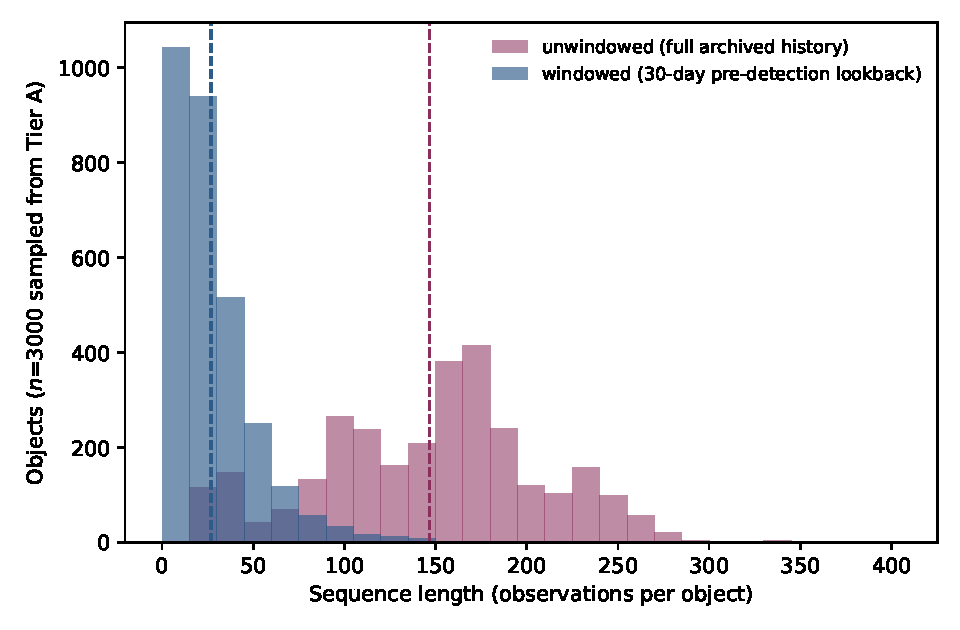
\includegraphics[width=0.72\linewidth]{figures/fig3_windowing_histograms}
\caption{Per-object sequence length, unwindowed (full archived history)
versus windowed (30-day pre-detection lookback), for the same
\WindowNSampleObjects{}-object stratified Tier A sample. Dashed lines mark
each distribution's mean. Windowing does not merely shorten sequences
uniformly; it collapses the distribution onto the much shorter range a
live alert stream actually produces.}
\label{fig:windowhist}
\end{figure}

This left-edge window bounds only how far back a sequence may reach. It
does not bound how far \emph{forward} a sequence may extend, and for a
fading transient this rarely matters -- the object drops below the
detection threshold and its own last detection arrives naturally soon after
its first. For a recurring or continuously variable source, nothing fades,
so a sequence's right edge sits wherever the underlying simulation happened
to end, independent of anything resembling a supernova's characteristic
timescale. Table~\ref{tab:spans} reports this directly, computed from the
raw ELAsTiCC2 exotic-class model directories: a tidal disruption event
(TDE, a bounded, fading transient) has a mean detection span of
\ExoticSpanMeanTDE{} days, while an eclipsing binary (EB) and a changing-look
AGN (CLAGN) -- both continuously variable, non-fading sources -- have mean
spans of \ExoticSpanMeanEB{} and \ExoticSpanMeanCLAGN{} days respectively,
\ExoticSpanRatioEB{}--\ExoticSpanRatioCLAGN{}$\times$ longer, despite a per-object observation count only
\ExoticNobsMeanEB{}--\ExoticNobsMeanCLAGN{} versus TDE's \ExoticNobsMeanTDE{}
(about \ExoticNobsRatioEB{}--\ExoticNobsRatioCLAGN{}$\times$, not \ExoticSpanRatioEB{}--\ExoticSpanRatioCLAGN{}$\times$). The right edge is therefore
unbounded in practice for exactly the class of object a live serving system
will keep re-observing indefinitely.

\begin{table}[htb]
\centering
\caption{Mean/median detection span and mean observation count per object,
computed directly from the raw ELAsTiCC2 model directories for one fading
transient (TDE) and two continuously-variable, non-fading sources (EB,
CLAGN). Detection span is $\max{-}\min$ of an object's own detection-flagged
observation times; all three directories were read in full with zero
discarded objects.}
\label{tab:spans}
\begin{tabular}{lrrrr}
\toprule
Class & $N$ objects & Mean span (d) & Median span (d) & Mean NOBS \\
\midrule
TDE (fading) & \ExoticNObjectsTDE{} & \ExoticSpanMeanTDE{} &
  \ExoticSpanMedianTDE{} & \ExoticNobsMeanTDE{} \\
EB (non-fading) & \ExoticNObjectsEB{} & \ExoticSpanMeanEB{} &
  \ExoticSpanMedianEB{} & \ExoticNobsMeanEB{} \\
CLAGN (non-fading) & \ExoticNObjectsCLAGN{} & \ExoticSpanMeanCLAGN{} &
  \ExoticSpanMedianCLAGN{} & \ExoticNobsMeanCLAGN{} \\
\bottomrule
\end{tabular}
\end{table}

A right-edge cap, \texttt{max\_span\_days}, was added and ablated at
$\{100, 200, \text{uncapped}\}$ days, evaluated by inference only against
the already-trained Tier A checkpoint (Table~\ref{tab:spanablation}).
\SpanChosenDefault{} days gives the best full-cutoff macro-F1 among the two finite settings
tested, costs only \SpanTwoHundredCost{} macro-F1 relative to uncapped, and
truncates at most \SpanTwoHundredMaxAffected{}\% of any class's objects. This value, \SpanChosenDefault{} days, was
adopted as the default the serving path passes explicitly; the underlying
function's own parameter default is left unchanged (\texttt{None}, i.e.\
uncapped) so that no existing training or evaluation call site is affected
by the change. Capping CLAGN's window at \SpanChosenDefault{} days more than triples its
mean classifier entropy (from \ClagnEntropyUncapped{} to
\ClagnEntropyCapped{}) and pulls its mean maximum softmax probability down
from \ClagnMaxProbUncapped{} to \ClagnMaxProbCapped{}, on the same
\ClagnNObjects{}-object population -- a real, measurable step toward
appropriate uncertainty on an out-of-distribution input, though still short
of a genuinely in-distribution object's own baseline confidence
(Section~\ref{sec:discussion}).

\begin{table}[htb]
\centering
\caption{Right-edge span ablation, Tier A test set, full cutoff, inference
only against the existing trained checkpoint (no retraining under any
cap).}
\label{tab:spanablation}
\begin{tabular}{lrrrr}
\toprule
\texttt{max\_span\_days} & Macro-F1 & Ia affected & Ib/c affected & II affected \\
\midrule
100 & \SpanHundredMacroF{} & \SpanHundredAffectedIa{}\% & \SpanHundredAffectedIbc{}\% & \SpanHundredAffectedII{}\% \\
\textbf{200 (chosen)} & \SpanTwoHundredMacroF{} & \SpanTwoHundredAffectedIa{}\% & \SpanTwoHundredAffectedIbc{}\% & \SpanTwoHundredAffectedII{}\% \\
Uncapped & \SpanUncappedMacroF{} & 0\% & 0\% & 0\% \\
\bottomrule
\end{tabular}
\end{table}

\subsection{Flux calibration}

Every reader in this pipeline is responsible for converting its source's
native photometric convention onto one shared scale before a canonical
alert is ever constructed: the SNANA \texttt{FLUXCAL} convention, AB
zeropoint 27.5. ELAsTiCC2's simulated flux already sits on this zeropoint,
so its reader performs no conversion at all -- an exception specific to
that one source, not a template for any other reader. A real ZTF alert
instead carries a PSF-fit magnitude and uncertainty
(\texttt{magpsf}/\texttt{sigmapsf}) referenced against that \emph{specific
alert's own} photometric zeropoint, \texttt{magzpsci}, which was measured
to vary row to row (across the full Tier B corpus, and again independently
on one live-polled Fink alert packet). Treating \texttt{magzpsci} as a
fixed constant, rather than reading it per row, would introduce a
brightness-dependent calibration error rather than a uniform shift -- worst
in exactly the faint, early-time regime this pipeline is built to classify
early. The conversion is
\begin{align}
  \mathrm{flux}_\mathrm{raw} &= \mathrm{sign} \times 10^{-0.4(\mathrm{magpsf} - \mathrm{magzpsci})}, \\
  \mathrm{flux\_err}_\mathrm{raw} &= |\mathrm{flux}_\mathrm{raw}| \times \frac{\ln 10}{2.5} \times \mathrm{sigmapsf},
\end{align}
followed by a rescaling from \texttt{magzpsci} onto \texttt{FLUXCAL}
zeropoint 27.5, applied per row through one shared, tested helper every
non-SNANA reader calls:
\begin{equation}
  \mathrm{flux}_{27.5} = \mathrm{flux}_\mathrm{zp} \times 10^{(27.5 - \mathrm{zp})/2.5},
\end{equation}
the only direction that leaves $\mathrm{mag} = \mathrm{zp} - 2.5\log_{10}\mathrm{flux}$
unchanged; LSST's nanojansky fluxes (zeropoint 31.4) are rescaled the same
way. The signal-to-noise feature ($\mathrm{flux}/\mathrm{flux\_err}$) is
scale-invariant and survives a calibration bug of this kind unchanged,
since the erroneous zeropoint factor cancels in the ratio; the
absolute-flux feature does not, and carries a silent, brightness-dependent
distortion into training with no symptom that looks like an error. This
is not hypothetical: an earlier version of the helper applied the
reciprocal factor, and Section~\ref{sec:silentfailures} describes what it
did and how it was found.

\subsection{Training protocol}

Splits are assigned by object identifier (checked for duplicates), never by
observation, so no object's light curve is divided across splits. Tier A
training uses class-weighted cross-entropy (sqrt-dampened inverse-class-
frequency weights, applied mildly rather than fully rebalancing toward the
real sky rate -- Section~\ref{sec:discussion}), AdamW, and cosine-annealed
learning-rate decay (Appendix~\ref{sec:appendixa} gives every hyperparameter
in full). The Tier B fine-tune uses a two-phase, discriminative
learning-rate schedule: the GRU trunk is frozen for the first two epochs
(only the head, and, where present, the static branch, train, at a
comparatively high learning rate), then unfrozen for six further epochs at
a learning rate $100\times$ lower than the head's own. This asymmetry is
deliberate: the Tier A encoder is the only part of this model that has ever
seen a negative-flux input (Tier B is \TierBNegFluxFrac{}\% negative-flux by construction,
Section~\ref{sec:discussion}), and Tier B's small, positive-flux-only
training set must be allowed to adapt the model to real ZTF cadence and
noise characteristics without being allowed to overwrite what the trunk
already learned about an input regime Tier B cannot itself supply, but
which live Tier C traffic already has.

\subsection{Metrics}

Accuracy is not used as a reportable metric anywhere in this report: on
this project's own class balance (and more strongly on the real sky rate),
a classifier that always predicts the majority class scores well on
accuracy while carrying no useful information at all. Macro-F1 -- the
unweighted mean of each class's own F1 score -- is used instead throughout,
since it cannot be inflated by favouring the common class over the rare
one. Per-class precision, recall, PR-AUC, ROC-AUC, and expected calibration
error are reported alongside macro-F1 for a fuller per-class picture
(Section~\ref{sec:results}). Because this is fundamentally an
\emph{early}-classification problem (Section~\ref{sec:introduction}), the
primary reported figure throughout is macro-F1 as a function of days since
an object's own first detection (the ``phase cutoff''), not a single
end-of-light-curve number: a model that only performs well once a light
curve has fully played out is of limited use to a system whose entire
purpose is to flag an object for spectroscopic follow-up \emph{while} it is
still interesting.


\chapter{Results \& Analysis}
\label{sec:results}

\section{Main classification results}

Table~\ref{tab:mainresults} reports macro-F1 and Ia-vs-rest ROC-AUC for
every trained configuration, alongside a majority-class and a five-feature
logistic-regression baseline fit on each tier with the frozen evaluation
harness. Every Tier B number is measured on zeropoint-corrected photometry
(Section~\ref{sec:silentfailures}); fine-tuned Tier B rows are the mean over
\TierBNSeeds{} seeds with identical data and object order, so a difference
between configurations can be read against the seed-to-seed spread.

\begin{table}[htb]
\centering
\caption{Main classification results at the full light-curve cutoff.
Per-class F1 columns are Ia/Ib-c/II in order. Fine-tuned Tier B rows are
the mean over \TierBNSeeds{} seeds, with the standard deviation of
macro-F1 in parentheses; zero-shot rows are inference-only and
seed-independent. The deployed configuration is marked; its served
checkpoint is the seed-42 run (macro-F1 \DeployedMacroF{}, Ia-vs-rest
ROC-AUC \DeployedRocAucIa{}, Ib/c F1 \DeployedFIbc{}). Output probabilities
carry the training-set class prior, not the real sky prior
(Section~\ref{sec:discussion}).}
\label{tab:mainresults}
\small
\begin{tabular}{L{4.6cm}rrrrr}
\toprule
Configuration & Macro-F1 & ROC-AUC (Ia) & F1 Ia & F1 Ib/c & F1 II \\
\midrule
Tier A, majority class & \BaselineMajTierAMacroF{} & \BaselineMajTierARocAucIa{} &
  \BaselineMajTierAFIa{} & \BaselineMajTierAFIbc{} & \BaselineMajTierAFII{} \\
Tier A, logistic regression & \BaselineLRTierAMacroF{} & \BaselineLRTierARocAucIa{} &
  \BaselineLRTierAFIa{} & \BaselineLRTierAFIbc{} & \BaselineLRTierAFII{} \\
Tier A, LC-only & \TierLCOnlyMacroFFull{} & \TierLCOnlyRocAucIaFull{} &
  \TierLCOnlyFIaFull{} & \TierLCOnlyFIbcFull{} & \TierLCOnlyFIIFull{} \\
Tier A, LC+static & \TierLCStaticMacroFFull{} & \TierLCStaticRocAucIaFull{} &
  \TierLCStaticFIaFull{} & \TierLCStaticFIbcFull{} & \TierLCStaticFIIFull{} \\
Tier A, LC+static, no photo-$z$ & \TierLCStaticNoPhotozMacroFFull{} &
  \TierLCStaticNoPhotozRocAucIaFull{} & \TierLCStaticNoPhotozFIaFull{} &
  \TierLCStaticNoPhotozFIbcFull{} & \TierLCStaticNoPhotozFIIFull{} \\
Tier A, WHXE head & \TierWHXEMacroFFull{} & \TierWHXERocAucIaFull{} &
  \TierWHXEFIaFull{} & \TierWHXEFIbcFull{} & \TierWHXEFIIFull{} \\
\midrule
Tier B, majority class & \BaselineMajTierBMacroF{} & \BaselineMajTierBRocAucIa{} &
  \BaselineMajTierBFIa{} & \BaselineMajTierBFIbc{} & \BaselineMajTierBFII{} \\
Tier B, logistic regression & \BaselineLRTierBMacroF{} & \BaselineLRTierBRocAucIa{} &
  \BaselineLRTierBFIa{} & \BaselineLRTierBFIbc{} & \BaselineLRTierBFII{} \\
Tier B, zero-shot, LC-only weights & \ZeroShotLCOnlyMacroF{} &
  \ZeroShotLCOnlyRocAucIa{} & \ZeroShotLCOnlyFIa{} & \ZeroShotLCOnlyFIbc{} &
  \ZeroShotLCOnlyFII{} \\
Tier B, zero-shot, LC+static weights & \ZeroShotMacroF{} &
  \ZeroShotRocAucIa{} & \ZeroShotFIa{} & \ZeroShotFIbc{} & \ZeroShotFII{} \\
Tier B, LC-only fine-tune & \LCOnlyMacroF{} (\LCOnlyMacroFSD{}) &
  \LCOnlyRocAucIa{} & \LCOnlyFIa{} & \LCOnlyFIbc{} & \LCOnlyFII{} \\
Tier B, LC+static fine-tune \textbf{(deployed)} & \WithStaticMacroF{}
  (\WithStaticMacroFSD{}) & \WithStaticRocAucIa{} & \WithStaticFIa{} &
  \WithStaticFIbc{} & \WithStaticFII{} \\
Tier B, LC+static+DRB fine-tune & \WithStaticDRBMacroF{}
  (\WithStaticDRBMacroFSD{}) & \WithStaticDRBRocAucIa{} & \WithStaticDRBFIa{} &
  \WithStaticDRBFIbc{} & \WithStaticDRBFII{} \\
\bottomrule
\end{tabular}
\end{table}

The sim-to-real gap is measured between matched configurations, so that it
isolates the change of data rather than a change of model. For the
deployed LC+static configuration it is
$\TierLCStaticMacroFFull{} \to \WithStaticMacroF{}$, a drop of
$\SimToRealGapStatic{}$ macro-F1; for LC-only it is
$\TierLCOnlyMacroFFull{} \to \LCOnlyMacroF{}$, a drop of
$\SimToRealGapLCOnly{}$. Both are the expected direction: simulated data has
no instrument noise, no real-bogus artifacts, and no mislabelled hosts, so
it is strictly easier than reality, and a model that scored identically on
both would be the stronger signal of a broken (leaking) evaluation split,
not of a better model. Fine-tuning recovers $\TransferGain{}$ macro-F1 over
the matching zero-shot model for LC+static
($\ZeroShotMacroF{} \to \WithStaticMacroF{}$) and $\TransferGainLCOnly{}$ for
LC-only ($\ZeroShotLCOnlyMacroF{} \to \LCOnlyMacroF{}$) -- fine-tuning is
doing real, measurable work, not re-labelling an already-adequate zero-shot
model. Host features help on both tiers: by $\PhotozGainWith{}$ macro-F1 on
Tier A and by $\StaticGainTierB{}$ on Tier B, \StaticGainOverSD{} times the larger of
the two configurations' seed-to-seed standard deviations, which is why
LC+static is the deployed configuration.

\section{Phase curve}

\begin{figure}[htb]
\centering
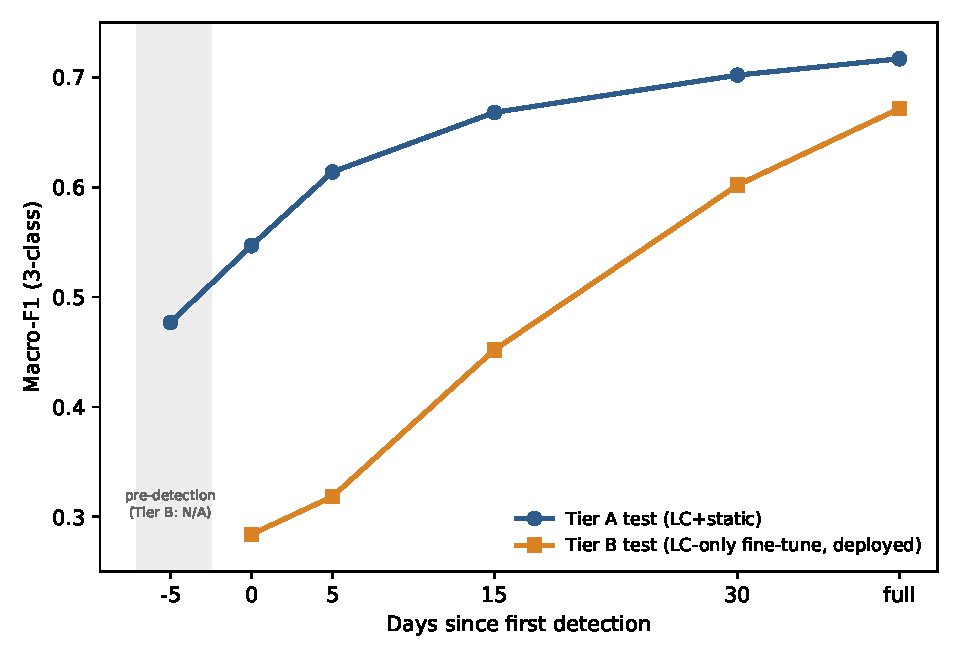
\includegraphics[width=0.78\linewidth]{figures/fig4_phase_curve}
\caption{Macro-F1 as a function of days since first detection, Tier A test
(LC+static) against Tier B test (LC+static fine-tune, the deployed
checkpoint; every point, including the full cutoff, read from that one
run's own evaluation). Tier B has no pre-detection ($-5$\,d) point because
its source metadata contains no forced-photometry row type at all
(Section~\ref{sec:discussion}); the comparison is therefore restricted to
cutoffs $\geq 0$. Conflating ``the model degrades on real data'' with ``the
model was evaluated on an easier phase slice'' would compare a full Tier A
curve (which includes $-5$\,d) against a necessarily truncated Tier B one
and misstate the size of the sim-to-real gap for reasons that have nothing
to do with sim-to-real generalisation.}
\label{fig:phasecurve}
\end{figure}

Both curves in Figure~\ref{fig:phasecurve} rise monotonically with more of
the light curve observed, from \TierLCStaticMacroFZero{} (Tier A, $0$\,d) to
\TierLCStaticMacroFFull{} (full) and from \DeployedPhaseZero{} (Tier B, $0$\,d)
to \DeployedPhaseFull{} (full). A model that got \emph{worse} with more data
would itself indicate a bug -- leakage that only helps a truncated input,
or an architecture unable to use a long sequence -- so the monotonic shape
is a sanity check that passed, not merely a pleasant picture.

\section{Confusion matrices}

\begin{figure}[htb]
\centering
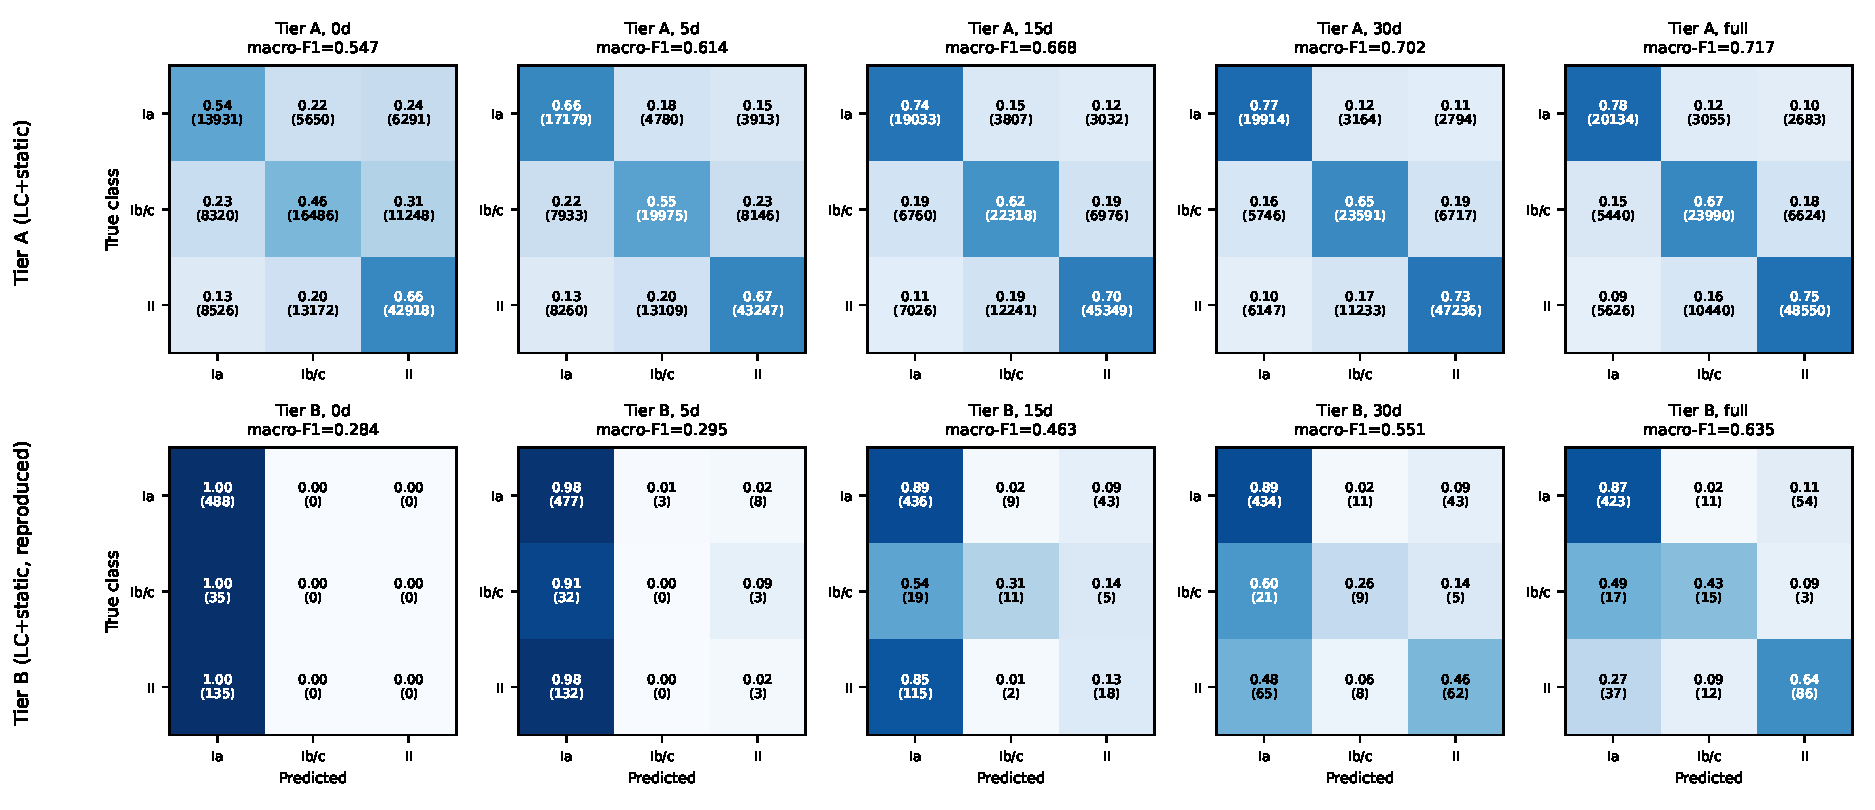
\includegraphics[width=\linewidth]{figures/fig5_confusion_grid}
\caption{Row-normalised confusion matrices (raw counts in parentheses) at
each phase cutoff. Top row: Tier A test, LC+static. Bottom row: Tier B
test, the deployed LC+static fine-tune (seed 42), read from that run's own
evaluation. At the earliest cutoffs the Tier B model predicts Ia for
\DeployedPhaseZeroPredIaFrac{}\% of objects at $0$\,d, the majority class;
the diagonal emerges as photometry accumulates.}
\label{fig:confgrid}
\end{figure}

\section{Prediction panels}

\begin{figure}[htb]
\centering
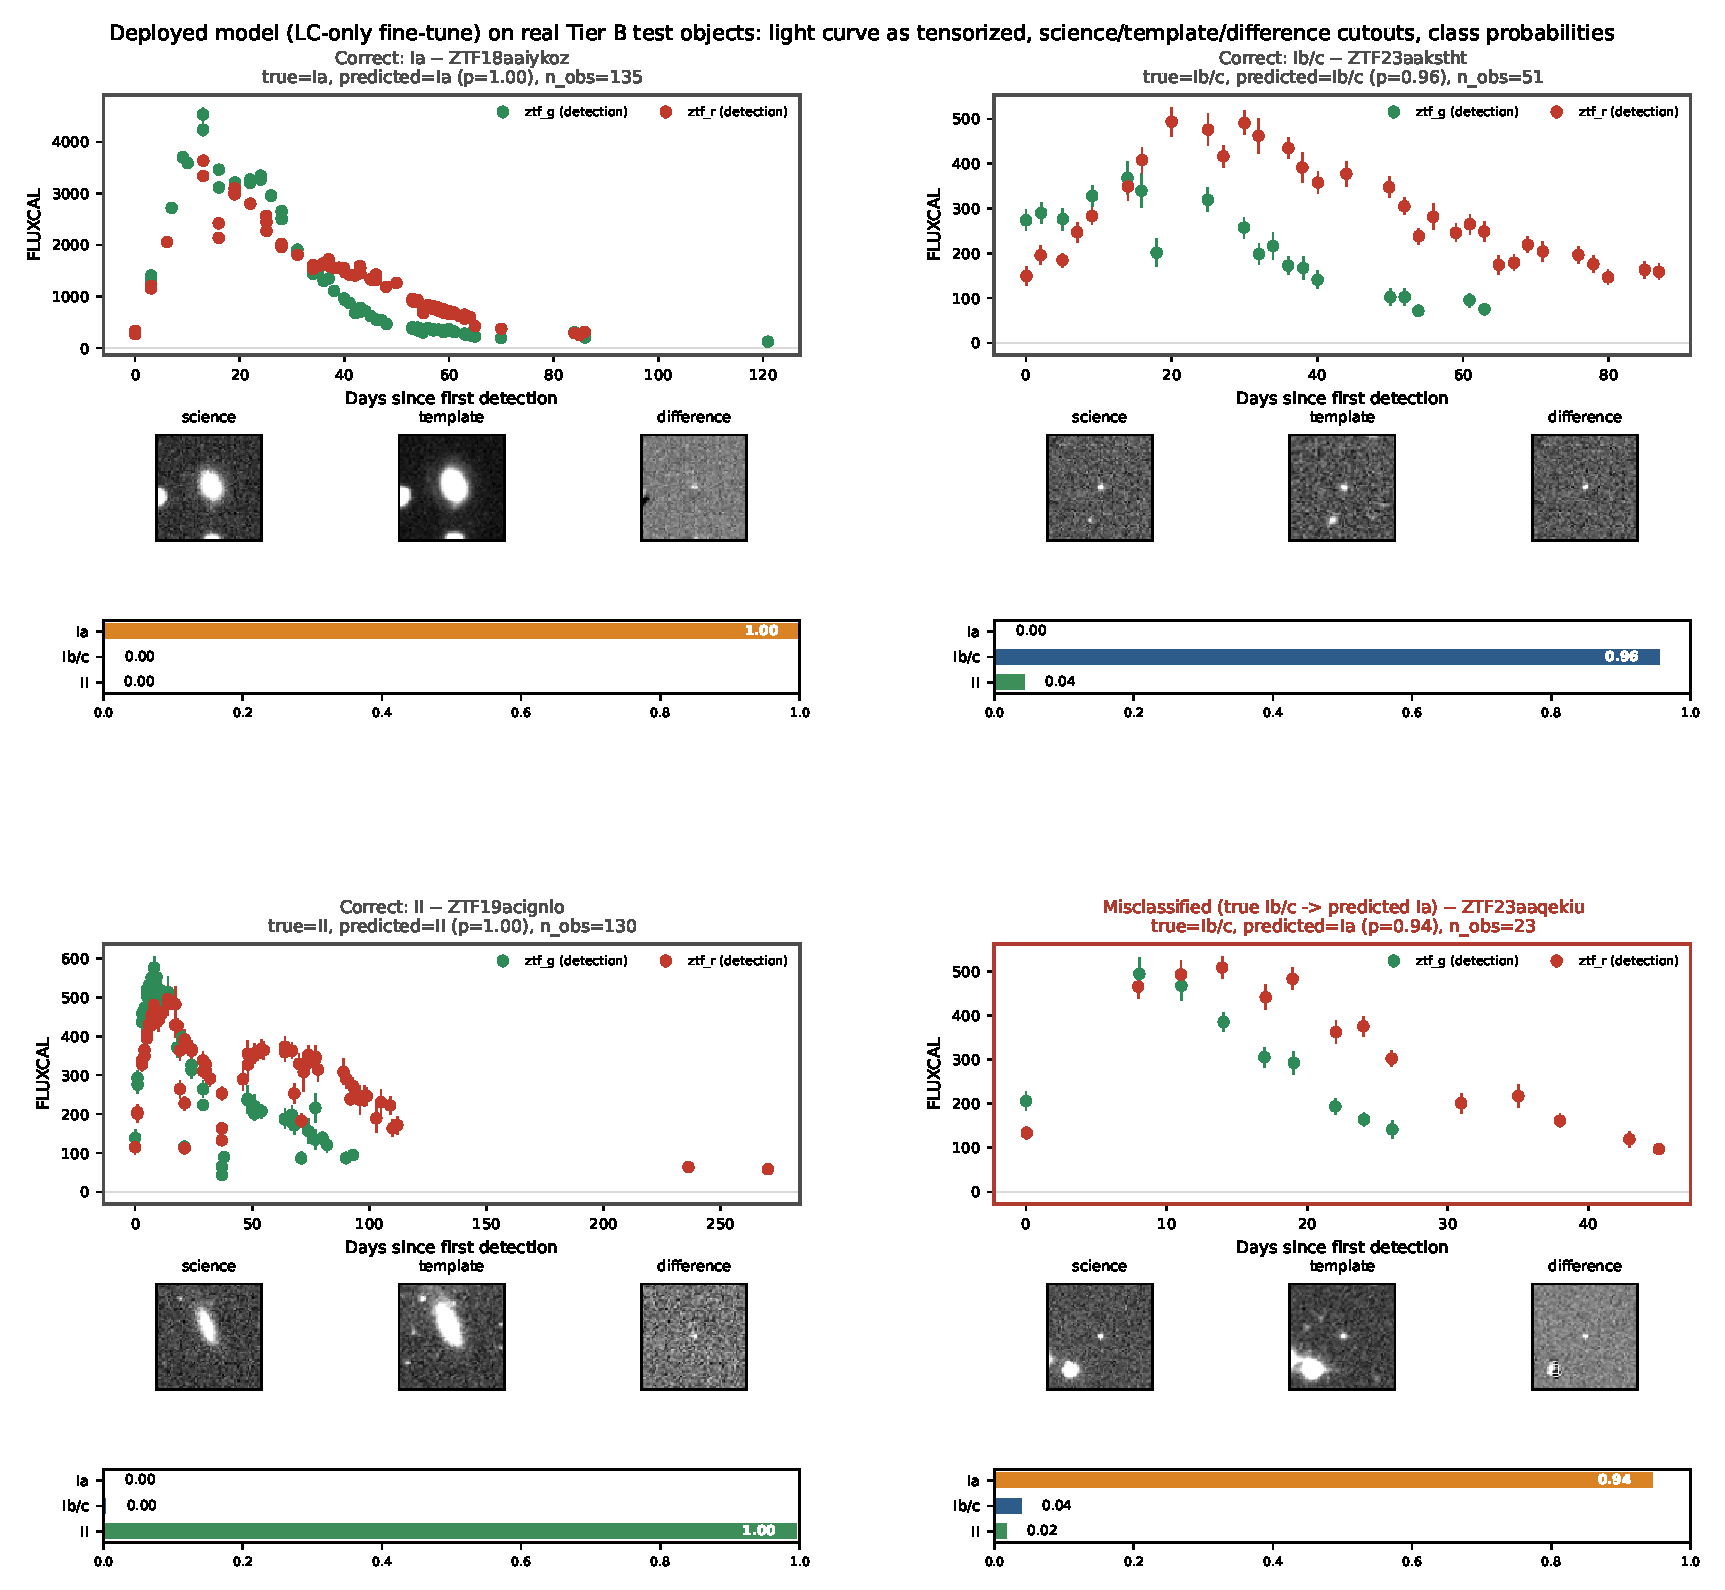
\includegraphics[width=0.92\linewidth]{figures/fig6_prediction_panels}
\caption{Four real Tier B test-split objects, run through the deployed
checkpoint (LC+static fine-tune) at inference time: the light curve as
tensorized (detections filled, forced photometry as small crosses, ZTF
$g$/$r$ in distinct colours), the real science/template/difference cutout
triplet (ZScale-rendered), and the model's own class-probability bars.
\emph{Selection}: for each class, the highest-confidence correctly
classified test object with at least \PanelMinObs{} observations (falling back to the
best available if no such object exists for a class); for the
misclassification panel, among test objects truly Ib/c but predicted Ia --
this project's own recorded dominant confusion -- the most confident wrong
call, tie-broken toward the sparser light curve. All four objects shown
were found by this selection rule on the first pass; none were
cherry-picked from a larger, unreported set of alternatives.}
\label{fig:predpanels}
\end{figure}

The misclassified panel in Figure~\ref{fig:predpanels} is instructive on
its own: a \PanelMisclassNObs{}-observation light curve is called Ia at
\PanelMisclassConfidencePct{}\% confidence while its spectroscopic type is
Ib/c -- exactly the kind of case the Ib/c F1 figure in
Table~\ref{tab:mainresults} summarises as a single number.

\section{Anomaly branch under domain shift}

\begin{figure}[htb]
\centering
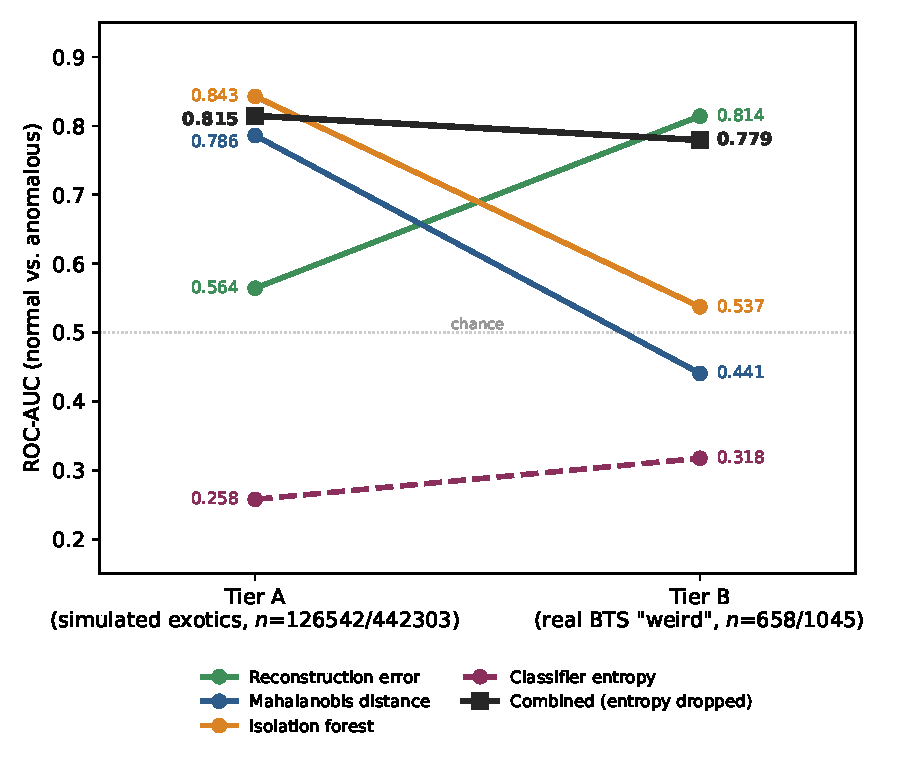
\includegraphics[width=0.62\linewidth]{figures/fig7_anomaly_slope}
\caption{Each anomaly-score component's normal-vs-anomalous ROC-AUC, Tier A
(simulated exotic classes held out of classifier training) against Tier B
(real, spectroscopically confirmed non-supernova BTS objects). The two
latent-space methods (isolation forest, Mahalanobis distance) fall toward
chance under the sim-to-real domain shift; reconstruction error rises. The
combined score (entropy dropped, black) is not the best score on either
individual set -- isolation forest alone beats it on Tier A, reconstruction
error alone beats it on Tier B -- but it is the only score that stays
useful on \emph{both}.}
\label{fig:anomalyslope}
\end{figure}

Table~\ref{tab:anomaly} gives the same comparison numerically, including
the combination with and without classifier entropy. Entropy was tested as
a fourth component and dropped: rather than being merely unhelpful, it was
actively \emph{harmful} to the combination on both evaluation sets, and its
own behaviour is the more interesting finding
(Section~\ref{sec:discussion}) -- it is markedly \emph{more} confident
(mean entropy \EntropyTierAExotic{} on Tier A's held-out exotic classes
versus \EntropyTierANormal{} on Tier A's own in-distribution test set; the
same direction, \EntropyTierBWeird{} versus \EntropyTierBNormal{}, on Tier
B) on objects the classifier has never seen anything like, exactly the
population an anomaly score is supposed to flag.

\begin{table}[htb]
\centering
\caption{Anomaly-component ROC-AUC (normal test objects vs.\ held-out
anomalous objects), each component and the combination with and without
classifier entropy. Tier B is scored on zeropoint-corrected photometry
with the same persisted scorers fitted on Tier A. The entropy-dropped
combination is recomputed directly from the per-object score files,
independently of the stored summary number, and agrees with it to four
decimal places. Before the zeropoint correction the Tier B entropy-dropped
combination was \PreFixAnomalyTierBCombinedThree{}.}
\label{tab:anomaly}
\begin{tabular}{lrr}
\toprule
Component & Tier A ($n$=\AnomalyTierANNormal{}/\AnomalyTierANAnomalous{}) &
  Tier B ($n$=\AnomalyTierBNNormal{}/\AnomalyTierBNAnomalous{}) \\
\midrule
Reconstruction error & \AnomalyTierAReconstructionError{} & \AnomalyTierBReconstructionError{} \\
Classifier entropy & \AnomalyTierAEntropy{} & \AnomalyTierBEntropy{} \\
Mahalanobis distance & \AnomalyTierAMahalanobis{} & \AnomalyTierBMahalanobis{} \\
Isolation forest & \AnomalyTierAIsoforest{} & \AnomalyTierBIsoforest{} \\
Combined (with entropy) & \AnomalyTierACombined{} & \AnomalyTierBCombined{} \\
\textbf{Combined (entropy dropped)} & \textbf{\AnomalyTierACombinedThreeRecomputed{}} & \textbf{\AnomalyTierBCombinedThreeRecomputed{}} \\
\bottomrule
\end{tabular}
\end{table}

\section{Gate D: the top-ranked anomalies}
\label{sec:gated}

The top \GateDNTotal{} of the pooled corrected Tier B evaluation set
(\AnomalyTierBNNormal{} normal supernovae and \AnomalyTierBNAnomalous{}
confirmed non-supernova objects), ranked by the deployed three-component
score, are \GateDNNoTreeNode{} cataclysmic variables, novae, luminous blue
variables or luminous red novae, \GateDNAGN{} AGN, \GateDNNinetyOneBG{}
91bg-like supernova and \GateDNTDE{} tidal disruption event;
\GateDNFromNormal{} come from the normal supernova population. Before the
zeropoint correction the same ranking gave \GateDPreFixNNoTreeNode{},
\GateDPreFixNAGN{}, \GateDPreFixNNinetyOneBG{} and \GateDPreFixNTDE{}
respectively, also with \GateDPreFixNFromNormal{} normal objects;
\GateDOverlapPreFix{} objects appear in both lists. The composition shifted
slightly toward AGN, but its character did not change. A photometric
heuristic built without pixel data tags \GateDNArtifactLike{} of the
\GateDNTotal{} as ``artifact-like'' (\GateDPreFixNArtifactLike{} before the
correction), but every one of them is a spectroscopically confirmed real
object, and inspection of the light curves shows multi-season sequences of
repeated outbursts or stochastic AGN variability rather than isolated
single-epoch spikes. The heuristic's label is a limitation of a proxy
without cutouts, not evidence of artifacts.

\section{Serving benchmarks}

The deployed LC+static model was benchmarked by replaying the full Tier B
test split (\ServingNAlerts{} alerts, \ServingNObjects{} objects) through the
complete Kafka~$\to$~Redis~$\to$~tensorize~$\to$~ONNX~$\to$~anomaly
score~$\to$~Postgres path, one alert at a time, with nothing else running.
Per-alert latency, from Kafka receipt to just before that alert's database
insert, is \ServingLatencyPFifty{}\,ms at the median,
\ServingLatencyPNinetyFive{}\,ms at the 95th percentile and
\ServingLatencyPNinetyNine{}\,ms at the 99th, at \ServingThroughput{}
alerts per second over the busy interval. The ONNX classifier on its own
takes \OnnxMsPerAlertBatchOne{}\,ms per alert at batch size one (median),
so the model is a small fraction of the per-alert cost; the remainder is
the unbatched Redis and Postgres round trips. Both figures are read from
stored benchmark artifacts. An earlier, lower-latency serving figure that
appears in this project's development log could not be matched to any
stored run and is not used. The same replay reproduces the offline
evaluation: the latest prediction per object scores macro-F1
\ReplayMacroF{} against the offline \DeployedMacroF{} for the same
checkpoint, a difference of \ReplayOfflineGap{} that comes from the
serving-only \SpanChosenDefault{}-day span cap.

\section{Live stream results}

\paragraph{ZTF.} With the corrected, deployed LC+static model, a
\LiveNovZtfElapsedMin{}-minute session on Fink's \texttt{fink\_sn\_\allowbreak candidates\_\allowbreak ztf}
topic received \LiveNovZtfNReceived{} alerts and scored all of them
(\LiveNovZtfNSkipped{} skipped) through the unmodified replay-mode pipeline,
covering \LiveNovZtfNObjects{} objects. Negative-flux detections, which are
absent from Tier B by construction (BTS pre-filters to brightening
subtractions before a candidate reaches its public release), made up
\LiveNovZtfNegFluxFrac{}\% of live detections. The latest prediction per
object is Ia \LiveNovZtfRawIa{}\%, Ib/c \LiveNovZtfRawIbc{}\% and II
\LiveNovZtfRawII{}\%; these objects carry no labels, so this is a
prediction-shape observation, not an accuracy measurement
(Section~\ref{sec:limitations} discusses the class prior). An earlier pair
of live sessions, run before the zeropoint correction with the previous
model, exposed a real bug: an undersized, CCD-edge cutout stamp raised an
exception that discarded the alert's entire light curve, not merely its
cutout (\LiveZtfRunOneNSkipped{} of \LiveZtfRunOneNReceived{} alerts lost).
It was fixed to degrade to ``no cutout'' and confirmed at
\LiveZtfRunTwoNSkipped{} skips on the following session.

\paragraph{LSST.} The LSST reader first met real traffic in the
pre-correction audit, where every alert was rejected because the live
schema names declination \texttt{dec} rather than the \texttt{decl} the
reader expected. With that field and the zeropoint corrected, the reader
converts all \LsstArchiveNConverted{} of \LsstArchiveNPackets{} archived live
packets, and the AB magnitude of each triggering source is preserved
through the conversion to within \LsstArchiveMaxDmag{}\,mag. A
\LiveNovLsstElapsedMin{}-minute live session on
\texttt{fink\_most\_\allowbreak likely\_sn\_\allowbreak lsst} then received \LiveNovLsstNReceived{}
alerts and scored all of them (\LiveNovLsstNSkipped{} skipped), covering
\LiveNovLsstNObjects{} objects, through the same unmodified pipeline;
\LiveNovLsstNegFluxFrac{}\% of detections had negative flux. The latest
prediction per object is Ia \LiveNovLsstRawIa{}\%, Ib/c
\LiveNovLsstRawIbc{}\% and II \LiveNovLsstRawII{}\%. \textbf{These alerts are
unlabelled, so no accuracy claim is possible for LSST}: the result shows
that LSST photometry flows end to end on the corrected flux scale, not
that the classifier is right about it.

\section{Gate outcomes}

\begin{table}[htb]
\centering
\caption{Outcome of each pre-registered validation gate
(Table~\ref{tab:gates}).}
\label{tab:gateoutcomes}
\small
\begin{tabular}{L{0.8cm}L{6.0cm}L{7.2cm}}
\toprule
Gate & Criterion & Result \\
\midrule
A & Plausible light curves per class; negative flux present;
  BTS class ratio near published anchor & Passed
  (\TierANegFluxMin{}--\TierANegFluxMax{}\% negative flux across Tier A
  directories; \TierBJoinRatio{}:1 Ia:Ib/c) \\
B & Shuffled labels collapse to chance; causal truncation-invariance;
  ROC-AUC within pre-registered band & Passed \\
C & Measurable sim-to-real accuracy drop & Passed
  ($\SimToRealGapStatic{}$ macro-F1 for LC+static, $\SimToRealGapLCOnly{}$
  for LC-only, matched configurations) \\
D & Top-\GateDNTotal{} ranked anomalies are artifact-dominated (\GateDArtifactAnchorPct{}\% anchor,
  \citealp{malanchev2021}) & \textbf{Deferred, not passed or failed}: the
  top \GateDNTotal{} on corrected Tier B (\GateDNNoTreeNode{} confirmed
  non-tree-node real classes, \GateDNAGN{} AGN, \GateDNNinetyOneBG{} 91bg,
  \GateDNTDE{} TDE; \GateDNFromNormal{} from the normal supernova test set)
  are spectroscopically confirmed real objects only, because the only
  evaluation population available was pre-filtered by construction at two
  separate stages (Section~\ref{sec:gated}) -- there was no bogus/artifact
  candidate in the pool for the ranker to have possibly found \\
\bottomrule
\end{tabular}
\end{table}


\chapter{Discussion}
\label{sec:discussion}

\section{The sim-to-real gap}

The sim-to-real drop is measured between matched configurations:
$\SimToRealGapStatic{}$ macro-F1 for the deployed LC+static model
($\TierLCStaticMacroFFull{} \to \WithStaticMacroF{}$) and
$\SimToRealGapLCOnly{}$ for LC-only
($\TierLCOnlyMacroFFull{} \to \LCOnlyMacroF{}$). It is read here as a
result, not a failure: Tier A carries none of Tier B's instrument noise,
real-bogus artifacts, or host-catalogue error, so a model that scored the
same on both would be the stronger evidence of a broken, leaking evaluation
split, since nothing about Tier B should be \emph{easier} than its own
simulated approximation. Part of the gap is a plain brightness mismatch:
real BTS objects are far brighter than the simulated training population
(Section~\ref{sec:limitations}). The transfer gains over the matching
zero-shot models ($+\TransferGain{}$ for LC+static, $+\TransferGainLCOnly{}$
for LC-only) show that fine-tuning is not cosmetic: a model carrying only
Tier A weights, evaluated on Tier B with no adaptation at all, is
measurably worse than one given even a small amount of real labelled data.

\paragraph{Ib/c misses its pre-registered band.} Before any Tier B result
existed, this project expected Ib/c F1 between \IbcBandLow{} and
\IbcBandHigh{}. The deployed configuration reaches \WithStaticFIbc{} (mean
over seeds; \DeployedFIbc{} for the served checkpoint), and LC-only reaches
\LCOnlyFIbc{}: both are below the band. The band is reported unchanged and
the miss is reported as a miss. Two reasons are likely, neither of which
would justify moving the band after the fact. First, the Tier B test split
holds only \TierBSupportIbc{} Ib/c objects against \TierBSupportIa{} Ia, so a
handful of objects moves this F1 substantially. Second, the band was
derived from published models trained and evaluated with far more Ib/c
examples than the \TierBJoinCountIbc{} spectroscopically confirmed Ib/c
objects available here across all splits. Before the zeropoint correction
this figure was \PreFixWithStaticFIbc{} for LC+static and
\PreFixLCOnlyFIbc{} for LC-only, inside the band, but those values came from
mis-scaled input and are not evidence that the band was met.

\section{Host features help on both tiers}

With correctly scaled fluxes, host and static features improve
classification on both tiers: by $\PhotozGainWith{}$ macro-F1 on Tier A
($\TierLCOnlyMacroFFull{} \to \TierLCStaticMacroFFull{}$) and by
$\StaticGainTierB{}$ on Tier B ($\LCOnlyMacroF{} \to \WithStaticMacroF{}$,
\StaticGainOverSD{} times the larger seed-to-seed standard deviation).
LC+static is therefore the deployed configuration.

An earlier version of this analysis reported the opposite on Tier B -- host
features making real-data fine-tuning worse -- and treated it as an open
finding. That inversion was an artifact of the flux-zeropoint conversion
error described in Section~\ref{sec:silentfailures}. Under identical code,
seeds and object order, the old fluxes put LC-only
\OldFluxStaticInversion{} macro-F1 above LC+static
($\OldFluxLCOnlyMacroF{}$ against $\OldFluxWithStaticMacroF{}$); the
corrected fluxes reverse the order. There is no remaining inversion to
explain.

Separately, on Tier A only, retraining LC+static without host photometric
redshift keeps \PhotozGainFractionSurviving{}\% of the static-feature gain
($+\PhotozGainWithout{}$ macro-F1 without photo-$z$, against
$+\PhotozGainWith{}$ with it): photo-$z$ contributes, but most of the Tier A
benefit comes from the other host fields.

\section{Windowing: one mechanism, three symptoms}

The train/serve sequence-length mismatch (Section~\ref{sec:windowing}), the
unbounded right edge for non-fading sources (Table~\ref{tab:spans}), and
classifier entropy's inversion under domain shift are one mechanism
observed at three points, not three separate findings. A model trained on
windowed sequences averaging \WindowMeanSeqLenWindowed{} observations
(Figure~\ref{fig:windowhist}) meets, at serving time, a changing-look AGN
whose uncapped tensorized sequence runs to a mean of \ClagnSeqLenUncapped{}
observations -- an input far outside anything the encoder was ever fit
against. The measured consequence is not increased uncertainty but
increased, misplaced confidence: CLAGN's mean entropy under the uncapped
window (\ClagnEntropyUncapped{}) sits \emph{below} the Tier A in-distribution
test population's own baseline (\EntropyTierANormal{}), and capping the
window at \SpanChosenDefault{} days moves it substantially toward, though not all the way
to, that baseline (\ClagnEntropyCapped{}). The general lesson is that a live
serving pipeline needs a bounded, \emph{recent} window for any long-lived
source, not a window defined relative to first detection alone -- a
distinction this project's own span cap addresses for training-distribution
matching but does not, by itself, solve for a serving-time rolling window
(Section~\ref{sec:analysis}).

\section{Confidently wrong on out-of-distribution input}

Table~\ref{tab:entropybyclass} makes the general pattern explicit across
every held-out simulated exotic class: mean entropy is markedly lower --
i.e., the classifier is more confident -- on several classes it was never
trained to recognise than on its own in-distribution test population
(\EntropyTierANormal{}). This is precisely the failure mode an anomaly
detector exists to catch, and precisely why classifier confidence cannot be
the component that catches it: a component that becomes \emph{more}
confident, not less, on the population it is meant to flag will actively
mislead a combination that trusts it, which is exactly what dropping it
measurably improved (Table~\ref{tab:anomaly}).

\begin{table}[htb]
\centering
\caption{Mean classifier entropy per held-out Tier A exotic class (computed
directly from the per-object entropy values already scored for the anomaly
branch, grouped by taxonomy id), against the Tier A in-distribution test
population's own baseline. CLAGN, the class with by far the longest
detection span (Table~\ref{tab:spans}), is also the most confidently wrong;
KN, a genuinely fast transient despite being outside the 3-class target
set, shows no inversion at all.}
\label{tab:entropybyclass}
\begin{tabular}{lrr}
\toprule
Population & $N$ & Mean entropy \\
\midrule
Tier A test (in-distribution) & \AnomalyTierANNormal{} & \EntropyTierANormal{} \\
KN & \ExoticNKN{} & \ExoticEntropyKN{} \\
CART & \ExoticNCART{} & \ExoticEntropyCART{} \\
SLSN & \ExoticNSLSN{} & \ExoticEntropySLSN{} \\
uLens & \ExoticNuLens{} & \ExoticEntropyuLens{} \\
ILOT & \ExoticNILOT{} & \ExoticEntropyILOT{} \\
TDE & \ExoticNTDE{} & \ExoticEntropyTDE{} \\
PISN & \ExoticNPISN{} & \ExoticEntropyPISN{} \\
CLAGN & \ExoticNCLAGN{} & \ExoticEntropyCLAGN{} \\
\bottomrule
\end{tabular}
\end{table}

\section{Anomaly components under domain shift}

The two latent-space methods (isolation forest, Mahalanobis distance) do
not survive the shift from simulated to real data because the latent space
they operate on is the Tier A encoder's own -- and that geometry simply
does not transfer to real ZTF objects the encoder never saw a shred of
during training. Reconstruction error moves the other way, because it
measures something closer to the physical light curve itself: a
cataclysmic variable or nova genuinely does not resemble a supernova's
flux-versus-time behaviour, a property of the raw signal that survives
exactly the domain shift that breaks the two latent-geometry methods. The
combination should be read as \emph{robustness under domain shift}, not as
peak performance -- it is beaten by the single best component on each
individual set (isolation forest on Tier A, reconstruction error on Tier B)
and is the only score that stays useful on both: its weaker value
(\AnomalyTierBCombinedThreeRecomputed{}, Tier B) is higher than the weaker of
the two values for any single component.
That is the honest, and more useful, claim to make about it.

\section{Systems findings}

The classifier itself is a small fraction of what an end-to-end serving
pipeline actually spends time on: ONNX inference takes
\OnnxMsPerAlertBatchOne{}\,ms per alert against a median end-to-end latency
of \ServingLatencyPFifty{}\,ms, which is dominated by the per-alert Redis
and Postgres round trips in this implementation
(Section~\ref{sec:results}). The implication for a broker-scale deployment is that
batching the state-layer writes, not further optimising the model, is the
obvious next lever if higher throughput is ever required.

\section{Validation findings: what would have failed silently}
\label{sec:silentfailures}

Table~\ref{tab:silentfailures} is, in its way, this report's methodological
contribution: every item in it would have produced a plausible, confident,
\emph{wrong} result, and none of them would have raised an error or crashed
anything.

The first row is qualitatively different from the rest, and it is the
strongest example of this section's argument. The project's governing
document described the conversion from a survey's native zeropoint to the
common FLUXCAL scale as a multiplication by a fixed factor, when the
correct operation is a division. That wrong value propagated into the
implementation, and then into the unit test written to verify the
implementation, which asserted the same factor. Implementation and test
agreed with each other and with the document, so all \TestsPassedPreFix{}
tests passed while every real ZTF flux was stored a median
\FluxBugFactor{} times too faint (\FluxBugFactorLow{}--\FluxBugFactorHigh{}
times across rows, since the ZTF zeropoint varies per exposure) and every
live LSST flux \LsstInversionFactor{} times too bright. A golden test is
only as independent as the number it was computed from; this one was
computed from the same wrong statement as the code. The replacement test
checks a property rather than restating a formula: the AB magnitude of a
source must be unchanged by the conversion. Once it existed,
\TestsFailedInvarianceOnOldCode{} tests failed against the old code. The
error survived every pre-registered gate because each Tier B result was
internally consistent -- fine-tuning, testing and serving all saw the same
mis-scaled fluxes -- and it surfaced only in comparisons across tiers,
where it produced a spurious finding (Section~\ref{sec:discussion}, host
features) and the wrong choice of deployed model.

\begin{table}[htb]
\centering
\caption{Silent-failure modes identified during development: what each was,
how it was caught, and what would have happened unchecked. None would have
raised an error.}
\label{tab:silentfailures}
\scriptsize
\begin{tabular}{L{2.7cm}L{4.6cm}L{5.8cm}}
\toprule
Issue & How it was caught & Consequence if unchecked \\
\midrule
Zeropoint conversion inverted in the governing document, the code and its
  test & A post-hoc audit checking AB-magnitude invariance numerically,
  after all \TestsPassedPreFix{} tests had passed & Real-data fluxes
  mis-scaled by an order of magnitude; a spurious ``host features hurt''
  finding and the wrong deployed model \\
Undocumented sentinel conventions (Table~\ref{tab:sentinels}) & Manual
  cross-check of raw FITS values against the format spec & Missing host
  features would train as real, extremely faint measurements \\
Three coexisting numbering schemes & Direct inspection found three
  different values for one object & Training against scrambled,
  meaningless class labels, indistinguishable from ``the model isn't
  learning'' \\
Full-history training data vs.\ a windowed live stream &
  Direct measurement of mean detections vs.\ forced photometry
  (Section~\ref{sec:windowing}) & A systematic train/serve distribution
  mismatch invisible in any offline metric, since the offline test split
  shares the training set's own (wrong) full-history shape \\
Unapplied/assumed-constant flux zeropoint & Per-row \texttt{magzpsci}
  variation measured directly on real data, not assumed constant &
  Silent, brightness-dependent flux error, worst in the faint early-time
  regime this project prioritises \\
A binary triage flag mistaken for a subtype label & Direct inspection of
  BTSbot metadata's column semantics before use & Training against ``is
  this a real transient at all,'' not the intended 3-class question,
  producing plausible-looking numbers for the wrong task \\
Inverted entropy component & Direct comparison of mean entropy,
  in-distribution vs.\ held-out anomalous, both tiers & A published
  anomaly score quietly worse than it needed to be, with no failure
  symptom pointing at entropy specifically \\
Undersized CCD-edge cutouts discarding an entire alert & A live ingestion
  run (Section~\ref{sec:results}), not offline testing & Live alerts'
  light curves discarded over an unrelated cutout-shape issue \\
\bottomrule
\end{tabular}
\end{table}

The common property across every row is that none of them would have raised
an error; each would have produced a confident, plausible, wrong result.
What caught them was not a single tool but reinforcing habits: a frozen
evaluation harness that could not be quietly adjusted to make a
disappointing number look better (Section~\ref{sec:methodology}), golden
tests written against one hand-verified real object before the reader code
that would have to pass them existed, pre-registered gates
(Table~\ref{tab:gates}) defined before the results they judge, and -- the
lesson of the first row -- tests that check a physical invariant rather
than a transcribed constant. This is the project's actual methodological
contribution, and is presented as such rather than as an apology.

\section{Limitations}
\label{sec:limitations}

Real BTS objects are much brighter than the simulated training set: the
median detection flux is \FluxMedianTierB{} FLUXCAL on Tier B against
\FluxMedianTierA{} on Tier A, a factor of about \FluxBrightnessRatio{}. The
conversion error masked roughly \FluxBugFactor{} times of that difference
(the pre-fix Tier B median was \FluxMedianTierBPreFix{}), so the encoder
was fine-tuned with a frozen-trunk, low-learning-rate schedule chosen
before the true size of the brightness shift was visible. This mismatch is
a plausible contributor to the sim-to-real gap; it has not been isolated,
and no schedule designed for it was tried.

Tier B is a systematically cleaner slice of the real sky than a live
stream, not a representative sample of one: it is pre-filtered to
brightening subtractions before a candidate ever reaches its public
release (\TierBNegFluxFrac{}\% negative flux, against
\LiveNovZtfNegFluxFrac{}\% measured on live ZTF traffic), it contains no
forced-photometry row type at all, and its labels are drawn from a
magnitude-limited spectroscopic follow-up programme, not from LSST's own
future detection limit.

Output probabilities carry the deployed model's training prior, not the
sky prior. On \LiveNovZtfNObjects{} live ZTF objects the deployed model
predicts Ia \LiveNovZtfRawIa{}\%, Ib/c \LiveNovZtfRawIbc{}\% and II
\LiveNovZtfRawII{}\%; Ib/c sits below its real sky rate, consistent with the
low Ib/c recall above. A single multiplicative prior correction does not
repair this: dividing out the ELAsTiCC prior gives Ib/c
\LiveNovZtfElasticcIbcRangeLow{}--\LiveNovZtfElasticcIbcRangeHigh{}\%
across plausible sky priors, and dividing out the effective Tier B
fine-tuning prior (Ia \TierBEffectivePriorIa{}\%, Ib/c
\TierBEffectivePriorIbc{}\%, II \TierBEffectivePriorII{}\%) pushes II to
\LiveNovZtfTierBCorrII{}\%. Calibrating the output probabilities is a
prerequisite for any rate estimate and has not been done.

LSST ingestion now works on real traffic (Section~\ref{sec:results}), but
LSST alerts carry no labels, so no accuracy claim is possible for them,
and their cutout stamps (\LsstArchiveStampMin{}--\LsstArchiveStampMax{}
pixels on a side) do not fit the fixed cutout shape of the canonical
schema, so LSST cutouts are not stored. The image encoder was cut, not
deferred: Tier B image data was never loaded across the project, and no
schedule remained to build, fuse, and retrain around it once that became
clear. Gate D remains unresolved, for the reason given in
Table~\ref{tab:gateoutcomes}.


\chapter{Conclusion \& Future Work}
\label{sec:conclusion}

\section{Conclusions}

\begin{enumerate}
  \item A causal, wavelength-conditioned light-curve encoder with a
    host-galaxy static branch, trained on simulated LSST-like data and
    fine-tuned on real ZTF data, reaches $\WithStaticMacroF{}$ macro-F1 on
    real, held-out test data (mean of \TierBNSeeds{} seeds), a
    $\SimToRealGapStatic{}$ drop from the same configuration's simulated-data
    score of $\TierLCStaticMacroFFull{}$ (Table~\ref{tab:mainresults}).
  \item Fine-tuning on a comparatively small real labelled set
    (\TierBLabeledTrain{} objects) recovers $\TransferGain{}$ macro-F1 over
    the matching zero-shot, simulation-only model
    (Table~\ref{tab:mainresults}) -- the sim-to-real transfer strategy this
    project depends on is doing real, measurable work.
  \item Host-galaxy static features improve classification on both tiers,
    by $\PhotozGainWith{}$ macro-F1 on simulated data and $\StaticGainTierB{}$
    on real data, and LC+static is the deployed configuration. The
    opposite result reported in an earlier version of this analysis was an
    artifact of a flux-conversion error (Section~\ref{sec:discussion}).
  \item Ib/c F1 on real data, $\WithStaticFIbc{}$, misses the
    \IbcBandLow{}--\IbcBandHigh{} band pre-registered for it. The test split
    holds only \TierBSupportIbc{} Ib/c objects, and the band was derived from
    models with far more Ib/c support; the band is left unchanged and the
    miss is reported.
  \item An anomaly-detection ensemble combining reconstruction error,
    Mahalanobis distance, and an isolation forest reaches
    $\AnomalyTierACombinedThreeRecomputed{}$ ROC-AUC on held-out simulated
    exotic classes and $\AnomalyTierBCombinedThreeRecomputed{}$ on real,
    spectroscopically confirmed non-supernova objects
    (Table~\ref{tab:anomaly}) -- not the best score on either individual
    set, but the only one that stays useful on both.
  \item Classifier confidence is not a usable anomaly signal: it becomes
    \emph{more} confident, not less, on inputs unlike anything the model
    was trained on (Table~\ref{tab:entropybyclass}), and including it in
    the anomaly combination measurably hurt performance on both evaluation
    sets.
  \item The most consequential error in the project passed every test and
    every gate, because the specification, the code and the test all
    shared it. A test of a physical invariant -- that a conversion between
    flux scales must leave a source's magnitude unchanged -- caught it where
    tests of the transcribed formula could not
    (Section~\ref{sec:silentfailures}).
  \item The served pipeline ingests live ZTF and LSST alerts without
    modification, at a median per-alert latency of
    \ServingLatencyPFifty{}\,ms; the LSST alerts are unlabelled, so the
    classifier's accuracy on LSST is untested.
  \item Gate D, the manual inspection of top-ranked anomalies against a
    published real-bogus-artifact anchor, could not be meaningfully
    evaluated: every population available was pre-cleaned of bogus
    candidates before the ranker ever saw it, at two independent pipeline
    stages (Table~\ref{tab:gateoutcomes}).
\end{enumerate}

\section{Future Work}

In order of what would most directly close an open item in this report:
calibrating the classifier's output probabilities, without which no
class-rate estimate from live traffic is meaningful; a fine-tuning
schedule designed for the large brightness shift between simulated and
real objects; closing Gate D against a genuinely unfiltered (or
reject/candidate) alert stream; obtaining labels for LSST alerts so that
accuracy on LSST can be measured; handling LSST's variable-size cutout
stamps; revisiting WHXE now that Tier B fine-tuning has introduced a
genuine population of non-SN-like real objects for its hierarchy to be
tested against; and batching the serving state layer's per-alert database
round trips, since the classifier itself is not the throughput bottleneck.


\chapter*{Author Contributions}
\addcontentsline{toc}{chapter}{Author Contributions}

A.K.\ led the technical work: the data pipeline and readers, model
architectures and training, the evaluation harness, the anomaly-detection
branch, the serving layer, and the results dashboard. A.P.\ led the
theoretical and interpretive work: supernova progenitor physics and
classification, the taxonomy adopted in Section~\ref{sec:data}, the
astrophysical interpretation of the results in Section~\ref{sec:discussion},
and the literature survey in Section~\ref{sec:literature}. Both authors
contributed to writing this report.

\section*{Data and Code Availability}
\addcontentsline{toc}{section}{Data and Code Availability}

The pipeline's source code, configuration, tests, and this report's own
figure-generation scripts live in the project repository (\texttt{sn-classifier};
repository access is internal to the project team at the time of writing).
Public data sources used:
\begin{itemize}
  \item ELAsTiCC2 training sample (LSST DESC), public, no credentials
    required: \url{https://portal.nersc.gov/cfs/lsst/DESC_TD_PUBLIC/ELASTICC/ELASTICC2_TRAINING_SAMPLE_2/}.
  \item BTSbot v10 (Zenodo), \href{https://doi.org/10.5281/zenodo.10839691}{DOI 10.5281/zenodo.10839691}.
  \item BTS Sample Explorer (Caltech), \url{https://sites.astro.caltech.edu/ztf/bts/explorer.php}.
  \item Fink broker, \url{https://fink-broker.org}; live ZTF and LSST alert
    access via \texttt{fink-client}.
\end{itemize}


\clearpage
\addcontentsline{toc}{chapter}{References}
\bibliographystyle{plainnat}
\bibliography{refs}

\appendix
\chapter{Hyperparameters and training configuration}
\label{sec:appendixa}

\begin{table}[htb]
\centering
\caption{Tier A pretraining configuration (identical across the flat,
LC+static, LC+static-no-photo-$z$, and WHXE runs except where noted).}
\begin{tabular}{L{5.2cm}L{8.3cm}}
\toprule
Parameter & Value \\
\midrule
Seed & 42 \\
Train/val/test split & 0.70 / 0.15 / 0.15, stratified by class, by object id \\
Pre-detection window & 30.0 days \\
Batch size & 256 \\
Epochs & 15 \\
Optimiser & AdamW, learning rate $1\times10^{-3}$, weight decay $1\times10^{-2}$ \\
LR schedule & Cosine annealing, $T_\mathrm{max}=$ num.\ epochs \\
Class weighting & sqrt-dampened inverse frequency, normalised to mean 1 \\
LC encoder & 2-layer GRU, hidden size 128, dropout 0.2 \\
Static encoder (LC+static only) & MLP, hidden size 32, output size 16, dropout 0.2 \\
WHXE $\alpha$ (WHXE run only) & 0.5 \\
Phase cutoffs (evaluation) & $-5, 0, 5, 15, 30,$ full (days since first detection) \\
ECE bins & 15 \\
\bottomrule
\end{tabular}
\end{table}

\begin{table}[htb]
\centering
\caption{Tier B fine-tuning configuration (applied identically to every
fine-tuned variant: zero-shot, LC-only, LC+static, LC+static+DRB).}
\begin{tabular}{L{5.2cm}L{8.3cm}}
\toprule
Parameter & Value \\
\midrule
Seed & 42 \\
Phase 1 (epochs 1--2) & GRU trunk frozen; head (+static/DRB branch) at LR $3\times10^{-4}$ \\
Phase 2 (epochs 3--8) & Trunk unfrozen at LR $3\times10^{-6}$; head continues at $3\times10^{-4}$, cosine-annealed to 0 \\
Weight decay & $1\times10^{-2}$ \\
Batch size & 128 \\
Pre-detection window & 30.0 days (a documented no-op on Tier B; Section~\ref{sec:discussion}) \\
Phase cutoffs (evaluation) & $0, 5, 15, 30,$ full (Tier B has no pre-detection point) \\
\bottomrule
\end{tabular}
\end{table}

\begin{table}[htb]
\centering
\caption{Anomaly-branch reconstruction-decoder training configuration.}
\begin{tabular}{L{5.2cm}L{8.3cm}}
\toprule
Parameter & Value \\
\midrule
Seed & 42 \\
Fit subsample & 60{,}000 Tier A objects, 3 normal classes only \\
Epochs & 5 \\
Batch size & 256 \\
Optimiser & AdamW, learning rate $1\times10^{-3}$, weight decay $1\times10^{-2}$ \\
Encoder hidden size (frozen, Tier A LC-only checkpoint) & 128 \\
Decoder hidden size & 64 \\
Dropout & 0.2 \\
Mahalanobis ridge regularisation & $\varepsilon = 1\times10^{-3}$ \\
\bottomrule
\end{tabular}
\end{table}

\chapter{BTS raw type-string to taxonomy mapping}
\label{sec:appendixb}

\begin{table}[htb]
\centering
\caption{Complete BTS Sample Explorer raw \texttt{type} string to
taxonomy-id mapping. Where more than one raw string maps to the same id,
they are grouped on one row.}
\label{tab:btsmapping}
\scriptsize
\begin{tabular}{L{7.2cm}L{3.6cm}L{2.9cm}}
\toprule
Raw BTS type string(s) & Taxonomy id & Notes \\
\midrule
\texttt{SN Ia}, \texttt{SN Ia-91T} & 2222 (Ia) & 91T-like folds into Ia; no dedicated node \\
\texttt{SN Ia-91bg} & 2226 (91bg) & Dedicated node, not folded into 2222 \\
\texttt{SN Iax} & 2225 (Iax) & Dedicated node, not folded into 2222 \\
\texttt{SN Ib}, \texttt{SN Ic}, \texttt{SN Ic-BL}, \texttt{SN Ib/c} & 2223 (Ib/c) & \\
\texttt{SN II}, \texttt{SN IIn}, \texttt{SN IIP}, \texttt{SN IIL}, \texttt{SN IIb} & 2224 (II) & IIb is II, not Ib/c \\
\texttt{AGN} & 2332 (AGN) & Non-3-class, real taxonomy id \\
\texttt{SLSN-I}, \texttt{SLSN-II} & 2242 (SLSN) & Single undifferentiated node \\
\texttt{TDE}, \texttt{TDE-H-He}, \texttt{TDE-He}, \texttt{TDE-featureless} & 2243 (TDE) & \\
\texttt{ILRT} & 2244 (ILOT) & ILRT $\approx$ ILOT in the literature \\
\texttt{Ca-rich}, \texttt{SN Ca-rich-Ca} & 2245 (CART) & Moved from NO\_TREE\_NODE on review \\
\midrule
\multicolumn{3}{l}{\textit{Excluded from the 3-class set (\texttt{class\_id=None})}} \\
\midrule
\texttt{SN Ibn}, \texttt{SN Icn} & \texttt{excluded\_csm\_interacting} &
  Confirmed stripped-envelope, but judged CSM/interaction-powered
  photometrically; deliberately kept out of 2223 \\
\texttt{-}, \texttt{Other}, \texttt{other} & \texttt{unclassified} & No
  spectroscopic classification obtained yet -- missing data, not a
  confirmed negative \\
\texttt{CV?}, \texttt{AGN?} & \texttt{uncertain} & BTS's own tentative flag \\
\texttt{SN Ia-pec}, \texttt{SN II-pec}, \texttt{SN Ib-pec}, \texttt{SN Ic-pec}, \texttt{SN IIn-pec}, \texttt{SN Ia-CSM}, \texttt{SN Ia-SC} & \texttt{ambiguous} &
  Real spectra, family not specified unambiguously by the string alone \\
\texttt{CV}, \texttt{nova}, \texttt{LBV}, \texttt{LRN} & \texttt{no\_tree\_node} &
  Confirmed, unambiguous real classes with no matching taxonomy leaf \\
\bottomrule
\end{tabular}
\end{table}


\end{document}
